%%%%%%%%%%%%%%%%%%%%%%%%%%%%%%%%%%%%%%%%%%%%%%%%%%%%%%%%%%%%%%%%%%%%%%%%%%%%%%%%
%DIF LATEXDIFF DIFFERENCE FILE
%DIF DEL 2025_RAL_VPR_old/root.tex       Mon Jan 12 14:05:48 2026
%DIF ADD 2025_RAL_VPR_current/root.tex   Mon Jan 12 14:05:32 2026
%2345678901234567890123456789012345678901234567890123456789012345678901234567890
%        1         2         3         4         5         6         7         8

\documentclass[letterpaper, 10 pt, conference]{ieeeconf}  % Comment this line out if you need a4paper

%\documentclass[a4paper, 10pt, conference]{ieeeconf}      % Use this line for a4 paper

\IEEEoverridecommandlockouts                              % This command is only needed if 
                                                          % you want to use the \thanks command

\overrideIEEEmargins                                      % Needed to meet printer requirements.

\usepackage{acronym}
\usepackage{amsmath}
\usepackage{graphicx}
\usepackage{amssymb}
\usepackage{subcaption}
\usepackage{pifont}
\usepackage{algorithm}
\usepackage{algpseudocode}
\usepackage{booktabs}
\usepackage{multirow}
 \usepackage[margin=1.5cm]{geometry}
\newcommand{\cmark}{\ding{51}}
\newcommand{\xmark}{\ding{55}}

\usepackage{xcolor}
% glossary file
\acrodef{VPR}{Visual Place Recognition}
\acrodef{SeqSLAM}{Sequence SLAM}
\acrodef{HMM}{Hidden Markov Model}
\acrodef{LCD}{Loop Closure Detection}
\acrodef{DBoW2}{Discrete Bag of Words 2}
\acrodef{SLAM}{Simultaneous Localization and Mapping}
\acrodef{BoW}{Bag of Words}
\acrodef{SOM}{Self-Organizing Map}
\acrodef{GNG}{{Growing Neural Gas}}
\acrodef{GWR}{{Growing When Required}}
\acrodef{LARFSOM}{{Local Adaptive Receptive Field Self-Organizing Map}}
\acrodef{GCS}{{Growing Cell Structures}}
\acrodef{LARFSOM-ARC}{Local Adaptive Receptive Field Self-Organizing Map with Adjustable Resemblance for Category}
\acrodef{VLAD}{Vectors of Locally Aggregated Descriptors}
\acrodef{BMU}{Best Matching Unit}
\acrodef{ACVPR}{Adaptive Clustering for Visual Place Recognition}
\acrodef{SOM-TVS}{Self-Organizing Map with a Time-Varying Structure}

\acrodef{STM}{Short-term Memory}

%In case you encounter the following error:
%Error 1010 The PDF file may be corrupt (unable to open PDF file) OR
%Error 1000 An error occurred while parsing a contents stream. Unable to analyze the PDF file.
%This is a known problem with pdfLaTeX conversion filter. The file cannot be opened with acrobat reader
%Please use one of the alternatives below to circumvent this error by uncommenting one or the other
%\pdfobjcompresslevel=0
%\pdfminorversion=4

% See the \addtolength command later in the file to balance the column lengths
% on the last page of the document

% The following packages can be found on http:\\www.ctan.org
%\usepackage{graphics} % for pdf, bitmapped graphics files
%\usepackage{epsfig} % for postscript graphics files
%\usepackage{mathptmx} % assumes new font selection scheme installed
%\usepackage{times} % assumes new font selection scheme installed
%\usepackage{amsmath} % assumes amsmath package installed
%\usepackage{amssymb}  % assumes amsmath package installed

\title{\LARGE \bf
Spatio-temporal Self-organizing Visual Place Recognition*
}
\usepackage{caption} 
\usepackage{subcaption}
\usepackage{hyperref}
\author{Adriel F. L. A. da Silva$^{1}$, Aluizio F. R. Araújo$^{1}$, Adrien Durand-Petiteville$^{1}$, and Marcondes R. da Silva Júnior$^{1}$% <-this % stops a space
\thanks{*This work was supported by CAPES, ANR and FACEPE.}% <-this % stops a space
\thanks{Project repository available at: \url{https://github.com/notyriuss/matlab_larfsom}}
\thanks{$^{1}$All authors are with Centro de Informática, Universidade Federal de Pernambuco, Av. Jornalista Anibal Fernandes, s/n - Cidade Universitária, 50.740-560, Recife, PE, Brazil. {\tt\small aflas, aluizioa, adrien, mrsj@cin.ufpe.br}}%
}
%DIF PREAMBLE EXTENSION ADDED BY LATEXDIFF
%DIF UNDERLINE PREAMBLE %DIF PREAMBLE
\RequirePackage[normalem]{ulem} %DIF PREAMBLE
\RequirePackage{color}\definecolor{RED}{rgb}{1,0,0}\definecolor{BLUE}{rgb}{0,0,1} %DIF PREAMBLE
\providecommand{\DIFaddtex}[1]{{\protect\color{blue}\uwave{#1}}} %DIF PREAMBLE
\providecommand{\DIFdeltex}[1]{{\protect\color{red}\sout{#1}}}                      %DIF PREAMBLE
%DIF SAFE PREAMBLE %DIF PREAMBLE
\providecommand{\DIFaddbegin}{} %DIF PREAMBLE
\providecommand{\DIFaddend}{} %DIF PREAMBLE
\providecommand{\DIFdelbegin}{} %DIF PREAMBLE
\providecommand{\DIFdelend}{} %DIF PREAMBLE
\providecommand{\DIFmodbegin}{} %DIF PREAMBLE
\providecommand{\DIFmodend}{} %DIF PREAMBLE
%DIF FLOATSAFE PREAMBLE %DIF PREAMBLE
\providecommand{\DIFaddFL}[1]{\DIFadd{#1}} %DIF PREAMBLE
\providecommand{\DIFdelFL}[1]{\DIFdel{#1}} %DIF PREAMBLE
\providecommand{\DIFaddbeginFL}{} %DIF PREAMBLE
\providecommand{\DIFaddendFL}{} %DIF PREAMBLE
\providecommand{\DIFdelbeginFL}{} %DIF PREAMBLE
\providecommand{\DIFdelendFL}{} %DIF PREAMBLE
%DIF HYPERREF PREAMBLE %DIF PREAMBLE
\providecommand{\DIFadd}[1]{\texorpdfstring{\DIFaddtex{#1}}{#1}} %DIF PREAMBLE
\providecommand{\DIFdel}[1]{\texorpdfstring{\DIFdeltex{#1}}{}} %DIF PREAMBLE
\newcommand{\DIFscaledelfig}{0.5}
%DIF HIGHLIGHTGRAPHICS PREAMBLE %DIF PREAMBLE
\RequirePackage{settobox} %DIF PREAMBLE
\RequirePackage{letltxmacro} %DIF PREAMBLE
\newsavebox{\DIFdelgraphicsbox} %DIF PREAMBLE
\newlength{\DIFdelgraphicswidth} %DIF PREAMBLE
\newlength{\DIFdelgraphicsheight} %DIF PREAMBLE
% store original definition of \includegraphics %DIF PREAMBLE
\LetLtxMacro{\DIFOincludegraphics}{\includegraphics} %DIF PREAMBLE
\newcommand{\DIFaddincludegraphics}[2][]{{\color{blue}\fbox{\DIFOincludegraphics[#1]{#2}}}} %DIF PREAMBLE
\newcommand{\DIFdelincludegraphics}[2][]{% %DIF PREAMBLE
\sbox{\DIFdelgraphicsbox}{\DIFOincludegraphics[#1]{#2}}% %DIF PREAMBLE
\settoboxwidth{\DIFdelgraphicswidth}{\DIFdelgraphicsbox} %DIF PREAMBLE
\settoboxtotalheight{\DIFdelgraphicsheight}{\DIFdelgraphicsbox} %DIF PREAMBLE
\scalebox{\DIFscaledelfig}{% %DIF PREAMBLE
\parbox[b]{\DIFdelgraphicswidth}{\usebox{\DIFdelgraphicsbox}\\[-\baselineskip] \rule{\DIFdelgraphicswidth}{0em}}\llap{\resizebox{\DIFdelgraphicswidth}{\DIFdelgraphicsheight}{% %DIF PREAMBLE
\setlength{\unitlength}{\DIFdelgraphicswidth}% %DIF PREAMBLE
\begin{picture}(1,1)% %DIF PREAMBLE
\thicklines\linethickness{2pt} %DIF PREAMBLE
{\color[rgb]{1,0,0}\put(0,0){\framebox(1,1){}}}% %DIF PREAMBLE
{\color[rgb]{1,0,0}\put(0,0){\line( 1,1){1}}}% %DIF PREAMBLE
{\color[rgb]{1,0,0}\put(0,1){\line(1,-1){1}}}% %DIF PREAMBLE
\end{picture}% %DIF PREAMBLE
}\hspace*{3pt}}} %DIF PREAMBLE
} %DIF PREAMBLE
\LetLtxMacro{\DIFOaddbegin}{\DIFaddbegin} %DIF PREAMBLE
\LetLtxMacro{\DIFOaddend}{\DIFaddend} %DIF PREAMBLE
\LetLtxMacro{\DIFOdelbegin}{\DIFdelbegin} %DIF PREAMBLE
\LetLtxMacro{\DIFOdelend}{\DIFdelend} %DIF PREAMBLE
\DeclareRobustCommand{\DIFaddbegin}{\DIFOaddbegin \let\includegraphics\DIFaddincludegraphics} %DIF PREAMBLE
\DeclareRobustCommand{\DIFaddend}{\DIFOaddend \let\includegraphics\DIFOincludegraphics} %DIF PREAMBLE
\DeclareRobustCommand{\DIFdelbegin}{\DIFOdelbegin \let\includegraphics\DIFdelincludegraphics} %DIF PREAMBLE
\DeclareRobustCommand{\DIFdelend}{\DIFOaddend \let\includegraphics\DIFOincludegraphics} %DIF PREAMBLE
\LetLtxMacro{\DIFOaddbeginFL}{\DIFaddbeginFL} %DIF PREAMBLE
\LetLtxMacro{\DIFOaddendFL}{\DIFaddendFL} %DIF PREAMBLE
\LetLtxMacro{\DIFOdelbeginFL}{\DIFdelbeginFL} %DIF PREAMBLE
\LetLtxMacro{\DIFOdelendFL}{\DIFdelendFL} %DIF PREAMBLE
\DeclareRobustCommand{\DIFaddbeginFL}{\DIFOaddbeginFL \let\includegraphics\DIFaddincludegraphics} %DIF PREAMBLE
\DeclareRobustCommand{\DIFaddendFL}{\DIFOaddendFL \let\includegraphics\DIFOincludegraphics} %DIF PREAMBLE
\DeclareRobustCommand{\DIFdelbeginFL}{\DIFOdelbeginFL \let\includegraphics\DIFdelincludegraphics} %DIF PREAMBLE
\DeclareRobustCommand{\DIFdelendFL}{\DIFOaddendFL \let\includegraphics\DIFOincludegraphics} %DIF PREAMBLE
%DIF LISTINGS PREAMBLE %DIF PREAMBLE
\RequirePackage{listings} %DIF PREAMBLE
\RequirePackage{color} %DIF PREAMBLE
\lstdefinelanguage{DIFcode}{ %DIF PREAMBLE
%DIF DIFCODE_UNDERLINE %DIF PREAMBLE
  moredelim=[il][\color{red}\sout]{\%DIF\ <\ }, %DIF PREAMBLE
  moredelim=[il][\color{blue}\uwave]{\%DIF\ >\ } %DIF PREAMBLE
} %DIF PREAMBLE
\lstdefinestyle{DIFverbatimstyle}{ %DIF PREAMBLE
	language=DIFcode, %DIF PREAMBLE
	basicstyle=\ttfamily, %DIF PREAMBLE
	columns=fullflexible, %DIF PREAMBLE
	keepspaces=true %DIF PREAMBLE
} %DIF PREAMBLE
\lstnewenvironment{DIFverbatim}{\lstset{style=DIFverbatimstyle}}{} %DIF PREAMBLE
\lstnewenvironment{DIFverbatim*}{\lstset{style=DIFverbatimstyle,showspaces=true}}{} %DIF PREAMBLE
%DIF END PREAMBLE EXTENSION ADDED BY LATEXDIFF

\begin{document}



\maketitle
\thispagestyle{empty}
\pagestyle{empty}


%%%%%%%%%%%%%%%%%%%%%%%%%%%%%%%%%%%%%%%%%%%%%%%%%%%%%%%%%%%%%%%%%%%%%%%%%%%%%%%%
\begin{abstract}
% contextualizar
% falar sobre o desafio
% falar sobre o foco do trabalho
% falar sobre no que o modelo se destaca


In scenarios where a robot uses cameras as sensors to localize itself within a map built upon visual features, Visual Place Recognition (VPR) is essential, especially for relocation and loop closure detection. \DIFdelbegin \DIFdel{Nowadays, VPR computational cost remains a challenge especially }\DIFdelend \DIFaddbegin \DIFadd{Despite recent advances, VPR remains computationally challenging }\DIFaddend for long trajectories\DIFdelbegin \DIFdel{because matching time grows proportionally to the number of reference images}\DIFdelend \DIFaddbegin \DIFadd{, as matching time typically increases with the size of the reference database}\DIFaddend . To address this, we propose Spatio-temporal Self-organizing VPR (STS-VPR), a new VPR model processing spatio-temporal data to reduce computational burden while maintaining competitive accuracy across different environments. STS-VPR introduces Spatio-temporal Local Adaptive Receptive Field Self-organizing Map (ST-LARFSOM), a SOM with time-varying structure to cluster visual feature vectors, reducing the matching search, so that matching to occur only with the subset of reference images within the winner group. In addition, ST-LARFSOM has a short-term memory module to encode time-correlations of feature vectors reducing visual ambiguities. Moreover, a normalization operator yields consistent feature scaling. A high number of experiments suggest that STS-VPR achieves up to 42$\times$ faster matching than traditional approaches, while also improving overall precision, highlighting its potential for real-time robotic navigation in visually complex environments.


\end{abstract}


%%%%%%%%%%%%%%%%%%%%%%%%%%%%%%%%%%%%%%%%%%%%%%%%%%%%%%%%%%%%%%%%%%%%%%%%%%%%%%%%
\section{Introduction}

% Introduction to VPR and applications
\ac{VPR} is the task of matching a view of a place with a different view of the same place taken at a different time. To do so, query and reference images are typically transformed into visual features, then finding the image from the data set whose visual feature vector is the most similar to that of the query vector is the goal.
% \ac{VPR} is a task performed by an autonomous agent to determine which image in a database matches a query image. 
% Thus, \ac{VPR} can be seen as an image retrieval task in which each image has its geo-location tag identifying the place where the image was acquired. 
\ac{VPR} is essential for relocalization and \ac{LCD} in metric \ac{SLAM}~\cite{orbslam},  creation of topological maps~\cite{fabmap}, and for areas such as 3D reconstruction and augmented reality~\cite{whereisvpr}.

% show the evolution
% \ac{LCD} is a stage of SLAM systems aiming to vanish with accumulated errors over time to avoid significant distortions in the resulting map. 
%Pioneer \ac{VPR} solutions typically focused on exploring the different visual features to increase the matching accuracy. For example, handcrafted descriptors such as SIFT~\cite{sift} and SURF~\cite{surf} were employed by~\cite{dbow2}, showing promising performances for significant viewpoint changes.
% Such feature-based methods were often used in metric SLAMs for visual re-localization or \ac{LCD} in which they showed promising performances for great viewpoint changes. 
%However, such methods struggle with appearance changes, \textit{e.g.,} due to illumination or seasonal alterations~\cite{vprsurvey}. Despite numerous efforts to tackle that issue~\cite{whereisvpr,seqslam,vprsurvey}, the performance and robustness of \ac{VPR} models had a significant improvement when methods based on Convolutional Neural Networks (CNN) were proposed~\cite{netvlad, mixvpr, CosPlace, EigenPlaces}.
%

%
% show the problem
In robotics, \ac{SeqSLAM}~\cite{seqslam} marked a milestone in \ac{VPR}, accounting for the sequential nature of images captured by an autonomous agent and using sequence matching to incorporate temporal context. \ac{SeqSLAM} is robust to illumination and seasonal changes, but struggles with viewpoint variations and nonlinear trajectories, limitations partially mitigated with \ac{HMM}-based extensions~\cite{hmmseqslam}. \ac{SeqSLAM} was followed by Multi-Process Fusion~\cite{mpf}, in which sensor fusion improve \ac{VPR} accuracy. More recently, CNN-based models reached substantial improvements over the previous handcrafted methods, even so, the current \ac{VPR} approaches still take high computational costs since each query image is typically compared against the entire reference set, leading to a proportional increase in computations with dataset size, or they rely on Approximate Nearest Neighbors (ANN) to lessen computation~\cite{pair_vpr, transfvpr}, which often reduces accuracy.

\begin{figure}
    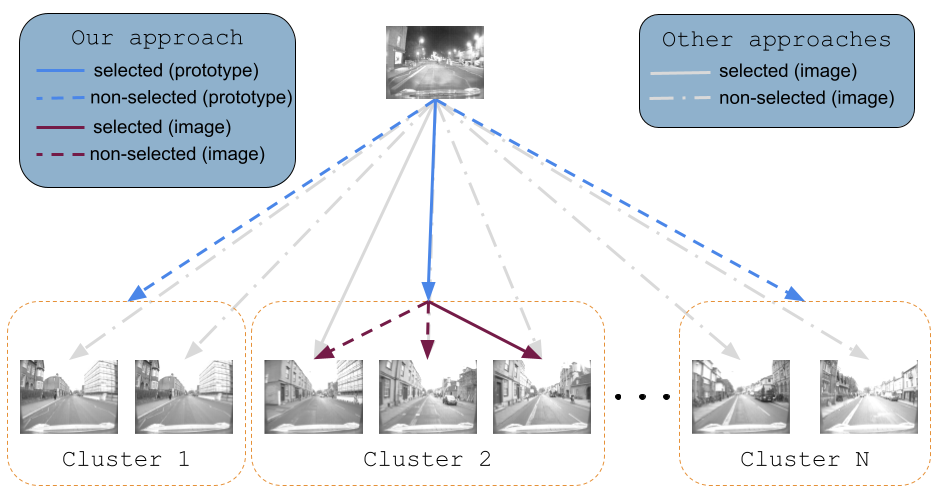
\includegraphics[width=\columnwidth]{images/model.png}
    \caption{Other approaches versus STS-VPR. Our approach restricts matching to the prototypes and clustered images.}
    \label{fig:our_method}
\end{figure}


% -> save it for latter
% Moreover, a \ac{VPR} method that can run in the robot without web connection and an incremental learning algorithm should also be a potential advance.

% show our solution to the problem: (1) solution, (2) what is G\ac{SOM} and for what it is used in ST-LARFSOM



In this work, we propose a modified version of \ac{LARFSOM}~\cite{larfsom} to reduce the computational cost of image matching through a clustering procedure for feature vectors with temporal-context allowing improvement of the recognition accuracy. During the training phase, the network clusters similar images and calculates a prototype for each cluster. Therefore, in the recognition stage, a query image is firstly compared to the set of prototypes, only then, to the images within the cluster of the most similar prototype, i.e. \ac{BMU} (Fig.~\ref{fig:our_method}); drastically reducing the number of comparisons necessary to identify the most similar image in the data set. \ac{LARFSOM} is a \ac{SOM-TVS} \cite{araujo2013self}, that can adapt its structure (architecture and topology) to incrementally acquire new knowledge over time, which makes it particularly suitable for online applications where information is continuously collected. 

For recognition of temporal sequences of images, we \DIFdelbegin \DIFdel{insert }\DIFdelend \DIFaddbegin \DIFadd{incorporate }\DIFaddend a \ac{STM} mechanism \DIFdelbegin \DIFdel{in }\DIFdelend \DIFaddbegin \DIFadd{into }\DIFaddend \ac{LARFSOM} \DIFdelbegin \DIFdel{aiming at disambiguation of }\DIFdelend \DIFaddbegin \DIFadd{to disambiguate visually }\DIFaddend similar reference images \DIFdelbegin \DIFdel{taken in different places based on such a }\DIFdelend \DIFaddbegin \DIFadd{captured at different locations by leveraging }\DIFaddend temporal retention \cite{oldtempsom3}. The main contributions of this paper are:

\begin{enumerate}
\item \textbf{Incremental learning}: The proposed model can acquire new knowledge without forgetting previous learning through the creation, elimination or adaptation of the clusters.
\item \textbf{STM module}: A simple STM module is inserted before the \ac{SOM-TVS} to encode spatio-temporal data, creating environment context for disambiguation.
\item \textbf{Normalization}: We apply a normalization process (after the STM module to avoid warping), such that all feature vectors are scaled dimension-wise based on the global minimum and maximum values of the reference set. The model saturates any query attribute that perchance is off the reference boundaries.
\item \textbf{Angular distance metric}: We use the angular distance between two vectors for determining the BMU. Such a distance is computationally cheaper than Euclidean distance with similar effectiveness.
%\item \textbf{Refinement stage}: After the initial clustering, a refinement step is performed in which LARFSOM is retrained using a weighting vector. This vector assigns different importance to each feature dimension based on its relative variability --- that is, dimensions with high variance relative to their mean are penalized, reducing their influence during similarity computation.

\end{enumerate}

The proposed enhancements over the LARFSOM pipeline for VPR not only enable a considerable reduction of matching time (up to 42 times faster as shown in Section IV), but they also ameliorate precision. Moreover, the STM module contributes by aiding the network to achieve even better performance. 

In the remainder of the paper, Section II presents the relevant works in terms of \ac{VPR} and \ac{SOM}; Section III details the STS-VPR model; and Section IV presents the results obtained with the proposed approach and compares its performance with state-of-the-art methods.


\section{Related Works}

The \ac{VPR} problem can be tackled with different tools, however, nowadays, there is a large use of approaches employing deep-learning feature extractors. We considered such a trend in combination with a \ac{SOM-TVS} equipped with a \ac{STM} mechanism, allowing incremental learning of spatio-temporal data.   

\subsection{CNN-based VPR models}

% Introduction to the VPR timeline
%The pioneer models on \ac{VPR} employed handcrafted descriptors such as SIFT~\cite{sift} and SURF~\cite{surf} to determine if two images correspond to the same place. 




% Applications in loop closure detection
%Among the most widely adopted approaches for \ac{LCD} are bag-of-words models, which encode a set of feature-based local descriptors into a compact vector representation. In ORB-SLAM, a representative instance of this family, DBoW2~\cite{dbow2}, is employed to perform \ac{LCD}, enabling the recognition of previously visited places.

% most recent research on VPR
Most recent research focus on CNN-based VPR models, with NetVLAD~\cite{netvlad}, which integrated a Vector of Locally Aggregated Descriptors (VLAD) layer and a weakly supervised training scheme for matching images of the same place over time. In turn,  CosPlace~\cite{CosPlace} and EigenPlaces~\cite{EigenPlaces} presented training strategies to handle viewpoint diversity and improve the inter-category separation, using backbones like ResNet or VGG. MixVPR~\cite{mixvpr} combines a pre-trained CNN with MLP-based feature aggregation for efficient and robust representation. As previously described, our approach clusters vectors of the CNN-based descriptors for matching. 

\subsection{Spatio-temporal Self-Organizing Networks}

Self-Organizing Maps (SOMs) were already previously employed to process spatio-temporal data to learn simultaneously spatial correlations and temporal dependencies between patterns. Voegtlin \cite{oldtempsom2} enumerated different approaches to handle time in SOMs, such as explicit representations, methods based on lateral connectivity, recurrent connections, leaky integrators, and combinations of these strategies. A pioneering approach was proposed by Kangas \cite{kangasthesis} that time-shifts each input vector and concatenates them to form an explicit temporal representation, which is then used as input to the SOM. Barreto and Araújo \cite{oldtempsom2} employed SOM for system identification using a self-supervised learning scheme. During training, the inputs are concatenated temporal vectors containing both input and its corresponding output components. At test time, each input vector is used to determine the winner: the model determines the distance between an input vector and all the parts of the prototypes vectors that represent the input, thus, the remaining prototype components (the output-dimensions) are taken as the SOM estimated output. Parisi et al. \cite{tempsom2} also address temporal information by weighting inputs based on previous inputs or previous BMUs, therefore, they introduced a global context array that combines past BMUs and inputs depending on prototype activations. Such a context is utilized for the determination of the BMU. Our approach, ST-LARFSOM also adopts spatio-temporal representations for solving VPR.


%%% removed to get space
%Such a model was then applied to 3D object detection and grasp synthesis, predicting pixel-wise antipodal grasp configurations \cite{tempsom3}.

\subsection{SOM-based VPR models}

%For real-time and resource constrained tasks in \ac{VPR} other metrics start to have a huge importance, such as computing time and memory. With that in mind, 
Cebollada et al.~\cite{evaluation} utilize SOMs for \ac{VPR} to reduce computation time with minimal accuracy loss by utilizing a hierarchical topological map. In their work, the position of the nodes is determined by the average position of the clustered images and the feature vector of the query image is compared with the weight of each node in the network, with the closest node determining the position. Da Silva et al. ~\cite{scmusom} use a more sophisticated SOM-based model. Instead of determining the positions of the nodes, it focuses solely on clustering the reference database involved in the matching process, thereby avoiding errors related to node position estimation, while still significantly reducing computation time. 

% Introducing why we use growing SOMs in this problem
%The \ac{SOM-TVS} represents an advancement over the traditional \ac{SOM} model, designed to address the limitations of a fixed and predetermined map structure. Unlike the conventional SOM, where the number of nodes and the topology of the map are predefined, \ac{SOM-TVS} dynamically adjusts these parameters during the learning process. During training, the map's topology is not static but is adjusted in response to the data distribution. This enables the map to more accurately represent the input distribution, enhancing the fidelity of the representation. These features make \ac{SOM-TVS} particularly effective for applications in dynamic environments where the data distribution evolves over time~\cite{araujo2013self}.

% LARFSOM
%The \ac{LARFSOM}~\cite{larfsom} is a self-organizing map model derived from \ac{GWR}, developed for image compression, retaining the competitive learning and clustering characteristics of the \ac{SOM}. It simplifies \ac{GWR} by updating only the best matching unit. Unlike \ac{GNG}, the \ac{LARFSOM} grows only when the activation value of a prototype is unsatisfactory, resulting in faster convergence.

% G\ac{SOM} topological map

%Besides that, specific \ac{SOM} structures known as \ac{SOM-TVS}~\cite{araujo2013self} have the useful property of being adaptable to new input data, allowing for easy modification of the \ac{SOM} network topology to account for new places in the \ac{VPR} task. 
Some models rely on \ac{SOM-TVS} structures for \ac{VPR}. Kazmi and Mertsching~\cite{gsom_vpr} introduced an approach that  updated the network online, while using node activations to estimate the agent’s current location and detect revisited places. Similarly, Zhang et al.~\cite{gsomapp1} employed a \ac{SOM-TVS}-based model to build cognitive maps by associating grid cell activations with visual information, thereby enabling place recognition. In those previous works the SOM updating occurs while an agent explores an environment whereas in our approach the learning stage is fully offline: the images are collected beforehand and then SOM is trained once. Such a characteristic makes our method more suitable in cases for which prior mapping is feasible, and when the goal is to exploit the clustering and prototype-based representation to reduce matching time.




%Baozhong Li et al.~\cite{sgsommap} introduce a neural network model based on an improved \ac{SOM} and grid cells (GCs) for bionic position estimation in unmanned vehicles. By leveraging grid cells' firing patterns and a two-level Self-Growing \ac{SOM} (SGSOM), the model decodes spatial information and adapts to environmental changes without prior training, making it effective for real-time autonomous navigation. This approach not only advances the biological understanding of animal navigation but also contributes to the development of sophisticated navigation systems for unmanned vehicles.


%HU et. al.~\cite{etm} introduces e-TM, a self-organizing neural %network framework for incremental topological mapping and %navigation, leveraging episodic memory and fusion adaptive resonance %theory (ART) networks. e-TM extracts salient landmarks from visual %observations, consolidates them into spatial memory, and generates %sparse topological graphs. It enables efficient navigation through %shortcut discovery and smoother movement by integrating human %demonstrations.

% ST-LARFSOM in relation to other models
%ST-LARFSOM adapts \ac{LARFSOM} to cluster gathered images for the \ac{VPR} task, maintaining low computational costs while achieving competitive performance compared to state-of-the-art methods.



\section{Spatio-temporal Self-organizing VPR (STS-VPR)}

%\begin{figure*}[t]
%    \centering
%    \begin{subfigure}{0.32\textwidth} % Ajuste a largura para caber lado a lado
%        \centering
%        
\includegraphics[width=\textwidth]{training_1.eps}
%        \caption{}
%        \label{fig:training_1}
%    \end{subfigure}
%    \hfill
%    \begin{subfigure}{0.32\textwidth}
%        \centering
%        
\includegraphics[width=\textwidth]{training_2.eps}
%        \caption{}
%        \label{fig:training_2}
%    \end{subfigure}
%    \hfill
%    \begin{subfigure}{0.32\textwidth}
%        \centering
%        
\includegraphics[width=\textwidth]{training_3.eps}
%        \caption{}
%        \label{fig:training_3}
%    \end{subfigure}
%    \caption{Illustration of different training configurations. The node prototypes are in red, the grey dots are the samples outside the activation thresholds, the blue dots are inside the activation thresholds and the green dot is the current sample. The green lines represent the distances to the 2 closest prototypes, the orange lines are the Voronoi diagram contours and the dashed black circles are the activation thresholds.}
%    \label{fig:training}
%\end{figure*}

\DIFdelbegin \DIFdel{ST-LARFSOM }\DIFdelend \DIFaddbegin \DIFadd{STS-VPR }\DIFaddend consists of three steps: (i) Preprocessing of incoming images, both
reference and query data sets; (ii) feature extraction with a chosen descriptor; and (iii)
visual place recognition based on visual characteristics. It is worth mentioning that to
create discriminating local representations, spatio-temporal vectors are generated
through a STM module that aims to avoid visual conflict. The proposed model creates clusters of contextualized images with the Spatio-temporal Local Adaptive Receptive Field Self-organizing Map (ST-LARFSOM), increasing the speed and accuracy of the VPR.

% The proposed model begins by extracting feature vectors from both reference and query images. These vectors are then passed through a causal discrete-time FIR filter to incorporate temporal context. The filtered outputs are subsequently normalized, as described in the first subsection.

% Following normalization, the model proceeds to cluster the reference feature vectors, assigning each cluster a representative prototype. This clustering process is performed in two stages. The first is the training stage, which follows the LARF\ac{SOM} pipeline~\cite{larfsom}, enhanced with a pruning strategy and a termination criterion. The second is a refinement stage, where weights are attributed to each feature vector's dimension.

% Once clustering is complete, each normalized query vector is compared only to the prototypes to determine its closest cluster. The model then searches for the most similar reference image within the winning cluster, avoiding exhaustive comparisons across all reference images. This selective strategy significantly reduces computational cost while, in general, improving the retrieval performance.


\subsection{Preprocessing}\label{sub:preprocessing}


In our VPR model, \DIFdelbegin \DIFdel{images, }\DIFdelend both reference and query \DIFdelbegin \DIFdel{, }\DIFdelend \DIFaddbegin \DIFadd{images }\DIFaddend are not directly used \DIFdelbegin \DIFdel{to perform the place recognitionbut rather }\DIFdelend \DIFaddbegin \DIFadd{for place recognition; instead, they are }\DIFaddend transformed into feature descriptors \DIFdelbegin \DIFdel{, }\DIFdelend $\mathbf{x} \in \mathbb{R}^{d}$, \DIFaddbegin \DIFadd{where }\DIFaddend $d$ \DIFdelbegin \DIFdel{is the problem dimension, and, then, they become }\DIFdelend \DIFaddbegin \DIFadd{denotes the descriptor dimensionality, yielding }\DIFaddend contextualized visual feature vectors. Initially, the input images are converted to the RGB color space\DIFdelbegin \DIFdel{(if not so) }\DIFdelend \DIFaddbegin \DIFadd{, if necessary, }\DIFaddend to ensure consistent representation across the dataset. Each image is then uniformly resized to a fixed resolution of $320 \times 320$ pixels \DIFdelbegin \DIFdel{in order }\DIFdelend to standardize the input size required by the network. Finally, \DIFdelbegin \DIFdel{the }\DIFdelend pixel values are normalized using the standard mean and standard deviation \DIFdelbegin \DIFdel{values commonly adopted for several }\DIFdelend \DIFaddbegin \DIFadd{commonly adopted by several visual }\DIFaddend descriptors, as in \cite{CosPlace, EigenPlaces, mixvpr}. This normalization step helps \DIFdelbegin \DIFdel{to ensures }\DIFdelend \DIFaddbegin \DIFadd{ensure }\DIFaddend compatibility with models \DIFdelbegin \DIFdel{that have been pretrained on a }\DIFdelend \DIFaddbegin \DIFadd{pretrained on }\DIFaddend large-scale image \DIFdelbegin \DIFdel{set}\DIFdelend \DIFaddbegin \DIFadd{datasets}\DIFaddend .



%\begin{figure}[H]
%    \centering
%    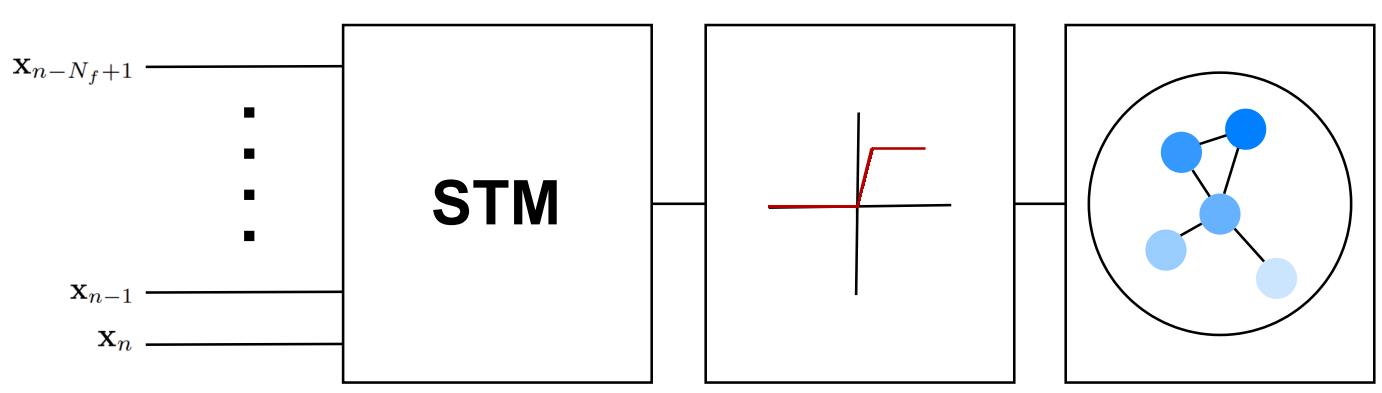
\includegraphics[width=1\linewidth]{images/model_diagram.png}
%    \caption{The Contextualized Visual Feature Vector is created when the visual
%features go through the STM (first module) and then, the values above one are
%clamped to one, and, then they are propagated towards the proposed SOM.}
%    \label{fig:diagram_model}
%\end{figure}

\subsection{Spatio-temporal Feature Construction}\label{sub:place_vector}

After the preprocessing phase, any descriptor, e.g., SIFT, SURF, VGG16, or ResNet, can be used for feature extraction, since the proposed method is visual feature agnostic, with only $d$ changing depending on the used descriptor. Next, each visual feature vector is combined by the STM module by a weighted exponential sum, to create a spatio-temporal feature vector, as shown in Eq.~\eqref{eq:filter}, denoted as $\mathbf{s}$. This representation aims to disambiguate similar single images by adding information from preceding images, capturing the temporal context in which an individual image is immersed.


\begin{equation}\label{eq:filter}
    \mathbf{s}_n = \sum\limits_{i = n}^{n-N_{f}+1} \alpha^{n - i} \mathbf{x}_{i}
\end{equation}

\noindent 
where $n$ indicates the current sampling instant, $N_{f}$ is the number of images to determine vector $\mathbf{s}$, and  $0 \le \alpha \le 1$ is a parameter weighting the importance of each visual feature vector, favoring recency. The combination of $n$ and $N_{f}$ determines the length of a sequence, and the importance of each feature belonging to it. Such a filter is applied to all  images to create \( \mathcal{S}^r = \{ \mathbf{s}^r_1, \mathbf{s}^r_2, \dots, \mathbf{s}^r_{N_r} \}  \) and \( \mathcal{S}^q = \{ \mathbf{s}^q_1, \mathbf{s}^q_2, \dots, \mathbf{s}^q_{N_q} \} \), the sets of reference and query spatio-temporal feature vectors. 


Each vector $\mathbf{s}$, from both $\mathcal{S}^r$ and $\mathcal{S}^q$, is component-wise normalized using the extrema values over \( \mathcal{S}^r \). To do it, we define $\mathcal{S}^r_k$, the set containing the $N_r$ values of the $k$-th element of the spatio-temporal features in $\mathcal{S}^r$, $\forall k \in  \mathbb{N}^+, 1 \leq k \leq d$. The minimum and maximum values for each dimension are:
%
$$
s^-_{k} = \min \mathcal{S}^r_k, \quad
s^+_{k} = \max \mathcal{S}^r_k
$$
%
Thus, $\bar{s}^{r}_{i,k}$, the normalized $k-th$ component of a reference spatio-temporal feature $\mathbf{s}^r_i$, $\forall i \in  \mathbb{N}^+, 1 \leq i \leq N_r$, is:

%
\begin{equation}
\bar{s}^{r}_{i,k} = \frac{s^r_{i,k} - s^-_{k}}{s^+_{k} - s^-_{k}}
\end{equation}
To ensures numerical stability in case of zero range in any component, $\bar{s}^{q}_{j,k}$, the normalized $k-th$ component of a query spatio-temporal feature $\mathbf{s}^q_j$, $\forall j \in  \mathbb{N}^+, 1 \leq j \leq N_q$, is given by:
\begin{equation}
\bar{s}^{q}_{j,k} =
\begin{cases}
\displaystyle \frac{s^q_{j,k} - s^-_{k}}{s^+_{k} - s^-_{k}}, & \text{if } s^+_{k} - s^-_{k} \ne 0 \\
0, & \text{otherwise}.
\end{cases}
\end{equation}

The normalization has the objective of equalizing the different dimensions of the
spatio-temporal features. Moreover, since reference an query features can be acquired
in very different visual contexts, for instance, acquisition at day light and recognition in
dark hours, the saturation module after the STM ensures that the spatio-temporal
features produced by the STM remain within a bounded range [0,1].


%Finally, the resulting spatio-temporal features $\bar{\mathbf{s}}^{r}_i$ and $\bar{\mathbf{s}}^{q}_j$ are L2-normalized. Such a process does not aim at increasing the relevancy of the spatio-temporal features but rather at facilitating faster similarity computation between two spatio-temporal features when using the cosine distance, as it's done by Amar Ali-bey et al.~\cite{mixvpr}.


\subsection{Training}\label{sub:training}

%\begin{algorithm}
%\caption{\textsc{LARFSOM}: Training Pseudocode}
%\label{alg:training}
%\scriptsize
%\begin{algorithmic}[1]
%\State \textbf{Input:} \( \mathcal{S}^{r,\text{norm}} \)
%\State \textbf{Output:} network
%\State Initialize network by choosing 2 random samples as prototypes

%\For{epoch = 1 to params.epochs}
%    \State Set \texttt{won\_in\_epoch} counter to zero for all prototypes
%    \State Randomly permute the training feature indexes
%    \State permuted\_training\_features $\gets$ permuted version of training\_features

%    \For{ \( i = 1, \dots, |\mathcal{S}^{r,\text{norm}}| \) }
%        \State in\_array $\gets$ permuted\_training\_features[i]
%        \State Update network using \texttt{main\_pipeline(in\_array, network, won\_in\_epoch)}
%    \EndFor

%    \State Prune network using \texttt{pruning(network)}

%    \If{termination criteria is met}
%        \State \textbf{break}
%    \EndIf
%\EndFor
%\end{algorithmic}
%\end{algorithm}

%\vspace{1em}

We proposed a spatio-temporal TVS SOM to deal with the VPR problem. Such a model integrates temporal context into each image representation; learns to cluster a huge number of time-contextualized images (tens of thousands) according to a predefined degree of similarity; creates new groups when the existing ones cannot cluster an image within a hypersphere centered in the group centroid; performs incremental learning for rapid acquisition of new knowledge without forgetting material previously learned; handles data extracted by different descriptors; and diminishes significantly the number of reference images compared with any query image. In sum, ST-LARFSOM can achieve competitive performance in comparison with the state-of-the-art methods whilst it reduces processing time. In ST-LARFSOM, each node represents a set of images from $\mathcal{\bar{S}}^r$ grouped according to a degree of similarity defined by a parameter called activation value $\phi$.



% The matching stage in the \ac{VPR} problem is addressed using a \ac{SOM}, which forms clusters over all reference feature vectors ($\boldsymbol{s^r_i}$) to determine the category of a given query feature vector ($\boldsymbol{s^q_j}$). These clusters are defined based on the similarity among reference samples. Once a query image is presented to the trained \ac{SOM} network, it assigns the image to a cluster (category), and recognition is achieved by identifying the reference image within that cluster that is most similar to the query.

% The VPR scenario commonly involves thousands of images that need to be clustered during training and thousands more to be recognized during inference. To handle this efficiently, we adopt a modified version of the \ac{LARFSOM} algorithm~\cite{larfsom}, aiming to achieve competitive performance with state-of-the-art methods, while significantly reducing processing time. Additionally, the learning strategy is incremental, allowing for fast and flexible training and retraining.

%%%%%%%%%%%%%%%%%%%%%%%%

The training is initialized by randomly selecting two spatio-temporal feature vectors from $\mathcal{\bar{S}}^r$. Each chosen vector is used to create a group giving values to their prototypes, the weight vectors ($\mathbf{w}$) associated to each cluster. A link between the nodes is inserted to make them topological neighbors. Then, the training proceeds iteratively: a spatio-temporal feature vector $\bar{\mathbf{s}}^{r}$ is randomly sampled from $\mathcal{\bar{S}}^r$, the distance between the input vector and the all prototypes is calculated, as shown in Eq.~\eqref{eq:distance}, to determine the closest prototype, also called the winner node. 

%
\begin{equation}
    \label{eq:distance}
    d(\mathbf{w}, \bar{\mathbf{s}}) = \mathbf{1} - \mathbf{w}^\top \bar{\mathbf{s}}
\end{equation}
%
The winner node ($c$) has its activation value calculated: 
%
\begin{equation}
    \label{eq:activation}
    \phi_{c}= e^{-d_{c}}
\end{equation}

If the computed activation value is greater than or equal to a predefined threshold $\phi_{th}$, the winner prototype is updated:

%
\begin{equation}
    \label{eq:prototype_update}
    \mathbf{w}^{new}_{c} = \mathbf{w}^{old}_{c} + \rho_f (\bar{\mathbf{s}} - \mathbf{w}^{old}_{c}),
\end{equation}

%
The learning rate $\rho_f$ is defined in Eq.~\eqref{eq:learning_rate}.
%
\begin{equation}
    \label{eq:learning_rate}
    \rho_f =
    \begin{cases}
        \rho^{v / v^+}, & \text{if } v \leq v^+, \\
        \rho,          & \text{otherwise}.
    \end{cases}
\end{equation}

\noindent
where $v$ denotes the number of wins of a prototype, and $v^+$ is a threshold
that prevents the learning rate from becoming excessively small, thereby
avoiding negligible updates.

If the activation value is below the threshold $\phi_{\text{th}}$, a new node is inserted in the map. Its prototype is equal to $\bar{\mathbf{s}}$, and its activation threshold is inherited from the original winner node. Finally, any previous connections between the new node and the top two winner nodes are removed, and new edges are formed between the two closest ones.  



This procedure is repeated throughout the training epochs. At the end of each epoch, the network is pruned by removing nodes with no connections or no wins during the whole training epoch. Training terminates when either the maximum number of epochs $N_e^+$ is reached or the relative unsupervised error falls below $\delta_{th}$ for $N_{err}$ consecutive epochs.



%%%%%%%%%%%%%%%%%%%%%%%%%%
%\subsubsection{Refinement}

%In this work, the vanilla \ac{LARFSOM} was modified and extended with a refinement stage. First, a vector $\mathbf{r} \in \mathbb{R}^{d}$ is used to weight the different dimensions during the distance calculation. Second, the network is retrained with a new epoch without pruning or growing. In this context, growing refers to the process of introducing new prototypes into the map, while pruning denotes the removal of empty or disconnected prototypes, as described before. Each element of  $\mathbf{r}$ is computed using Eq. \eqref{eq:r}, where $\mu_j$ and $\sigma$ are  the mean and standard deviation of the $j^{th}$ dimension respectively,$\forall j \in  \mathbb{N}^+, 1 \leq j \leq N_q$.
%
%\begin{equation}
%    \label{eq:r}
%    r_j = \frac{\mu_j}{\sigma_j}
%\end{equation}
%
%The refinement vector $\mathbf{r}$ is then normalized as shown in Eq. \eqref{eq:r_bar}.
%
%\begin{equation}
%    \label{eq:r_bar}
%    \bar{r}_j = \frac{r_j - \min\limits_{1 \leq k \leq d} r_k}{\max\limits_{1 \leq k \leq d} r_k - \min\limits_{1 \leq k \leq d} r_k}
%\end{equation}
%
%Finally, the normalized refinement vector is included in the distance computation as shown in Eq. \eqref{eq:distance_r} where $\circ$ represents the Hadamard product. 

%\begin{equation}
%    \label{eq:distance_r}
%    d(\mathbf{w}, \bar{\mathbf{s}}) = \mathbf{1} - (\bar{r} \circ \mathbf{w}^\top) \bar{\mathbf{s}},
%\end{equation}

% \noindent
% Hence, this new distance calculation is used for the refinement stage.

%As a result, dimensions that present a lower relative variability (i.e., smaller standard deviation compared to the mean) receive a higher weight in the distance computation. This increases their influence on the similarity evaluation, effectively penalizing mismatches along more stable dimensions, while reducing the impact of noisier ones.

%The motivation for introducing a refinement phase for this vector is to facilitate parameter tuning. At the beginning of training, the activation threshold ($\phi_{th}$) would otherwise be overly sensitive to the refinement vector. The refinement phase, therefore, is designed to perform small adjustments to the prototypes’ positions, functioning as a fine-tuning step.



\subsection{Recognition}\label{sub:recognition}

\begin{figure}[h]
    \centering
    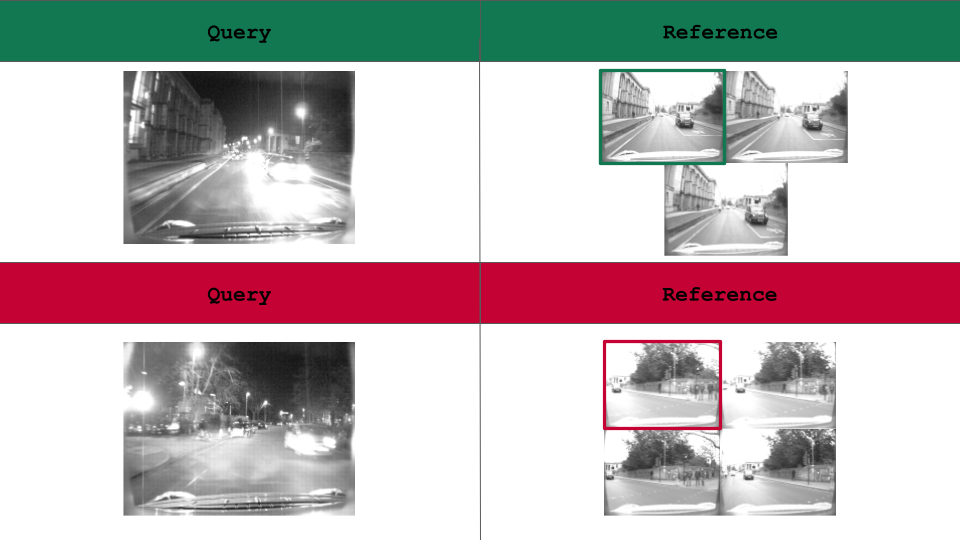
\includegraphics[width=1\linewidth]{images/testing.png}
    \caption{Example of right (in green) and wrong (in red) query–reference matches, showing multiple clustered reference images.}
    \label{fig:recognition}
\end{figure}




The training phase clusters the contextualized reference vectors, dividing the feature space of ST-LARFSOM into Voronoi regions. Thus, following a presentation of a query vector \(\bar{\mathbf{s}}^q \in \bar{\mathcal{S}}^q\), the group of the most similar prototype is found by Eq.~\eqref{eq:distance}. Then, ST-LARFSOM finds the reference image in the group that is the closest one to the query vector. Therefore, any query image is just compared with the images of a single group. Fig.~\ref{fig:recognition} illustrates an example of this recognition procedure. 



Based on by Milford and Wyeth~\cite{seqslam}, we compute a \emph{matching score} using the ratio between the best match inside a sliding window of size $\mathbf{\Delta}$ and the best match outside it. Our model employs the prototypes of the reference samples as components of the moving window. Fig.~\ref{fig:matching_window} describes how the \emph{matching score} ($\mu$) is calculated, which is essential to improve the mF1 metric (in Subsection~\ref{sub:results}). This procedure yields a confidence measure for validating matches and contributes to achieving higher precision at lower recall levels.

\begin{figure}[h]
    \centering
    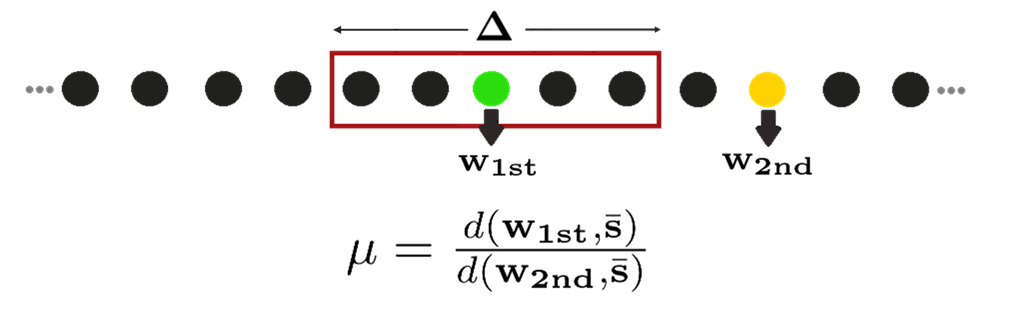
\includegraphics[width=\linewidth]{images/match_window.png}
    \caption{The window is formed around the winning prototype in order to separate its closest to its farthest prototypes. The variable $\mathbf{w_{1st}}$ represents the winning prototype, while $\mathbf{w_{2nd}}$ is the winning prototype outside the sliding window with size $\mathbf{\Delta}$.}
    \label{fig:matching_window}
\end{figure}






\section{Experiments and Results}



We present the experimental setup and the performance of the STS-VPR compared with consolidated and state-of-the-art models, namely, SCMuSOM~\cite{scmusom}, MixVPR~\cite{mixvpr}, CosPlace~\cite{CosPlace}, EigenPlaces~\cite{EigenPlaces}, SeqSLAM~\cite{seqslam}, and MPF~\cite{mpf}. The tests were performed on a computer equipped with an AMD Ryzen 7 processor and 80 GB RAM. A GEFORCE RTX 3060 GPU was only used for feature extraction.



\subsection{Data Sets}



%%%%%%%%%%%%%%%%%%%%%%%%%%%%%%
\begin{table*}[h]
\caption{Data sets characteristics.}
\label{tab:data set_characteristics}
\begin{tabular}{lccccccccc}
\hline

\multirow{3}{*}{Name} & \multirow{3}{*}{Role} & \multirow{3}{*}{File} & \multirow{3}{*}{Range} & Sampling & Number of& \multirow{3}{*}{Obs.} & Matching & High & High \\
 &  &  &  & Ratio & Images & & Threshold & Appearance & Viewpoint\\
 &  &  &  & & & & & Variation & Variation\\
\hline
%%%%%%%%%%%%
\multirow{2}{*}{St. Lucia}    & Ref. & 19/08/09 - 8:45 & 1-8000 & 1:2 & 4000 & Day & \multirow{2}{*}{20 m} & \multirow{2}{*}{\xmark} & \multirow{2}{*}{\xmark}\\
\cline{2-7}
                              & Query & 19/08/09 - 14:10 & 1-8000& 1:2  & 4000 & Afternoon &  & &\\
\hline
%%%%%%%%%%%%
\multirow{5}{*}{Oxford Robotcar}    & Ref. & 09/12/14 - left & 400-6550 & 1:3 & 2050 & Day & \multirow{5}{*}{40 m} & \multirow{5}{*}{\cmark} & \multirow{5}{*}{\xmark}\\
\cline{2-7}
                              & Query & 10/12/14 - left & 1750-7900& 1:3  & 2050 & Night &  & &\\
\cline{2-7}
                              & Ref. & 09/12/14 - left & 1-34128 & 1:1  & 34128 & Day &  & &\\
\cline{2-7}
                              & Query & 10/12/14 - left & 1-38315 & 1:1 & 38315 & Night &  & &\\
\cline{2-7}
                              & Query & 14/11/14 - left & 1-39760 & 1:1  & 39760 & Night &  & &\\
\cline{2-7}
                              & Query & 13/02/15 - left & 1-30001 & 1:1  & 30001 & Day &  & &\\
\hline
%%%%%%%%%%%%
\multirow{2}{*}{Kitti}        & Ref. & Sequence 02 left & 1-3999 & 1:1 & 3999 & Day & \multirow{2}{*}{10 m} & \multirow{2}{*}{\xmark} & \multirow{2}{*}{\xmark}\\
\cline{2-7}
                              & Query & Sequence 02 left & 4389-4619 & 1:1  & 230 & Day &  & &\\
\hline
%%%%%%%%%%%%
\multirow{2}{*}{Synthia}        & Ref. & Sequence 2 & 1-888 & 1:1 & 888 & Front camera & \multirow{2}{*}{80 m} & \multirow{2}{*}{\xmark} & \multirow{2}{*}{\cmark}\\
\cline{2-7}
                              & Query & Sequence 2 & 1-888 & 1:1  & 888 & Rear camera &  & &\\
\hline
%%%%%%%%%%%%
\multirow{2}{*}{Euroc}        & Ref. & Machine Hall 05 cam0 & 1-1599 & 1:1 & 1599 & Left camera & \multirow{2}{*}{3 m} & \multirow{2}{*}{\cmark} & \multirow{2}{*}{\cmark}\\
\cline{2-7}
                              & Query & Machine Hall 05 cam0 & 1600-2203 & 1:1  & 604 & Left camera &  & &\\
\hline
%%%%%%%%%%%%
\multirow{2}{*}{Pitts30k}        & Ref. & database & 1-10000 & 1:1 & 10000 & - & \multirow{2}{*}{25 m} & \multirow{2}{*}{\cmark} & \multirow{2}{*}{\cmark}\\
\cline{2-7}
                              & Query & queries & 1-6816 & 1:1  & 6816 & - &  & &\\
\hline
%%%%%%%%%%%%
\multirow{2}{*}{Nordland}        & Ref. & Summer & 1-35768 & 1:1 & 35768 & - & \multirow{2}{*}{10 images} & \multirow{2}{*}{\cmark} & \multirow{2}{*}{\xmark}\\
\cline{2-7}
                              & Query & winter & 1-35768 & 1:1  & 35768 & - &  & &\\
\hline
\end{tabular}   
\end{table*}

The compared methods were tested on seven data sets frequently used in the context of VPR and SLAM. Table \ref{tab:data set_characteristics} describes the various characteristics of the data sets. The reference and query sequences extracted from the St. Lucia data set \cite{st_lucia} are made of images taken along a same path during daylight. The Oxford Robotcar data set \cite{oxfordrobotcar}, in turn, is formed by sequences taken at night and during daylight. Moreover, three query sequences have more than 30,000 images, suitable for assessing the models for voluminous data sets. The Kitti data set \cite{kitti} contains images of an urban scenario with a high variety of viewpoints, similarly to cases occurring in loop closure detection. The Synthia data set~\cite{synthia} consists of a set of synthetic images of a simulated urban environment. The images acquired by the frontal camera are used as the reference, whereas the images from the back camera form the query sequences. The Euroc data set~\cite{euroc} is composed of images gathered by a drone inside a factory displaying significant differences such as high diversity in viewpoint and illumination. The Pitts 30k~\cite{pitts}, a subset of the Pittsburg data set, is formed by a collection of individual images in different places characterizing high viewpoint variation and visual aliasing. Finally, the Nordland data set~\cite{nordland} consists of video sequences captured from a train traversing the same route across different seasons. This data set is particularly useful for evaluating the robustness of visual place recognition under bold changes of image contents. 






%Maybe we should write a few words about the matching criteria.
The matching thresholds (Table \ref{tab:data set_characteristics}) were set to the previous choices in literature that vary according to the gathered positions data precision. Nevertheless, we chose 80 meters error tolerance for our tests with the Synthia data set, due to an existing visual offset for the query images~\cite{tolerance_synthia}.  All models in our experiments used this same threshold.



% for our experiments. Each data set differs from the others in at least one of the following aspects: degree of appearance change, number of reference and query images, time of day or season, urban versus rural environments, acquisition frequency, or whether the images were captured from ground-level or aerial perspectives. The variety of scenarios in which ST-LARFSOM is expected to perform is illustrated in Fig.~\ref{fig:qualitative}.

% Falar sobre lucia
% The St. Lucia data set~\cite{st_lucia} is composed of 10 sequences acquired at 15 frames per second. From these sequences, we sampled a sequence gathered at 8:45 am on 19/08/2009 used as the reference from the first to the 8,000-th frame, always skipping 1 frame, totaling 4,000 images. For the query, we chose the video sequence gathered at 14:10 on 19/08/2009. The 30 meters chosen by one of the previous models~\cite{mpf} was too high for doing a comparison between more recent models and ST-LARFSOM (due to different models easily reaching 100\% precision), so we chose a lower tolerance of 20 meters.

% Falar sobre Robotcar
% For the Oxford Robotcar~\cite{oxfordrobotcar}, the reference and query sequences were gathered on 09/12/2014 (day) and 10/12/2014 (night) respectively. In this case, we used the first 6,150 images, selecting 1 out of every 3 consecutive images; thus, we ended up with 2,050 images for both sequences. Moreover, we also tested the whole sequences without skipping any frame, using 10/12/2014 (night), 14/11/2014 (night), and 13/02/2015 (day) as queries. It is worth mentioning that we used the images acquired by the left front camera in our experiments. For this case, we took 40 meters tolerance as it was chosen by Stephen Hausler et al.~\cite{mpf}.

% Falar sobre o kitti
% Experiments with the Kitti data set~\cite{kitti} used images acquired by the left camera in ``sequence 02''. The reference sequence employed the first 3,999 images, while the query set was composed of the images 4,389 to 4,619. We aimed to test an urban scenario with high viewpoint variance similar to cases faced in loop closure detection. Considering GPS error and comparing the models with different tolerance values and noting that the order of the best to the worst model's performance does not change with this variation, 10 meters of tolerance was chosen.

% Falar sobre Synthia
% The Synthia data set~\cite{synthia} consists of a set of synthetic images of a simulated urban environment. Here, we selected the images from sequence 2, the summer scenario, for the experiments. Still, the images acquired by the frontal camera were used as the reference, whereas the images from the back camera formed the query set. For this data set, 80 meters error tolerance was chosen for our tests, giving the arguments from Garg et al.~\cite{tolerance_synthia}.

% % Falar sobre Euroc
% The Euroc data set~\cite{euroc} is composed of images gathered by a drone inside a factory displaying significant differences such as high variance in viewpoint and illumination. The utilized sequence was ``Machine Hall 05'', specifically the images from the left camera, with the last 604 frames used as query and the first 1,599 as reference images. Considering the ground truth noise and doing multiple tests with the different models, 3 meters of error tolerance were chosen for this data set in our tests.

% % Falar sobre Pittsburg

% The Pitts 30k~\cite{pitts}, a subset of the Pittsburg data set, is formed by a collection of individual images in different places characterizing high viewpoint variation and visual aliasing. Following the same default from previous papers~\cite{mixvpr,CosPlace,EigenPlaces}, 25 meters of error tolerance were chosen for this data set in our tests.

% % Falar sobre nordland
% The Nordland data set~\cite{nordland} consists of video sequences captured from a train traversing the same route across different seasons. This data set is particularly useful for evaluating the robustness of visual place recognition under strong appearance changes. In our experiments, we employed the summer sequence as the reference and the winter sequence as the query. All frames were extracted from the same forward-facing camera, focusing on testing the method’s capability to handle seasonal variations without significant viewpoint changes. For Nordland, as it was done by S{\"u}nderhauf et al.~\cite{nordland} 10 images of error tolerance were chosen for our tests.

\subsection{Models Setup}

Most STS-VPR parameters, including the recency factor ($\alpha$), unsupervised error threshold ($\delta_{th}$), number of epochs for which the error remains below $\delta_{th}$ ($N_{err}$), learning rate $\rho$, maximum number of victories $v^+$, maximum number of epochs $N_e^+$, and window size $\mathbf{\Delta}$, exhibited low sensitivity to variation. Therefore, the same values were used across all experiments $(\alpha = 0.85, \delta_{th} = 0.00878, N_{err} = 18, \rho = 0.5, v^+ = 100, N_e^+ = 1{,}000, \mathbf{\Delta} = 10)$. However, both the sequence length $N_{f}$ and the activation threshold \(\phi_{th}\) demonstrated high sensitivity to the characteristics of different environments and different descriptors. The sequence length was set to 15, and the values for \(\phi_{th}\), the most sensitive parameter, are shown in Table~\ref{tab:lhs}.\(\phi_{th}\) was determined to obtain a number of prototypes more or less equal to 20\% of the total number of reference samples. Indeed, the higher the value of \(\phi_{th}\) the higher the number of prototypes in ST-LARFSOM; improving the performances at the expense of computational endeavor. Such an improvement eventually saturates: additional prototypes no longer yield further performance gains. This is typically reached when the number of prototypes corresponds to approximately 15\% to 22\% of the total reference samples.

\begin{table}[h]
\centering
\caption{Activation threshold ($\phi_{th}$) values for each dataset and descriptor.}
\label{tab:lhs}
\resizebox{\columnwidth}{!}{
\begin{tabular}{l
                c
                c
                c
                c}
\toprule
\textbf{} & \textbf{MixVPR} & \textbf{Cosplace} & \textbf{Eigenplaces} & \textbf{ResNET} \\
\midrule
Robotcar       & 0.993 & 0.99  & 0.985 & 0.99  \\
Nordland       & 0.97  & 0.98  & 0.97  & 0.915 \\
Kitti          & 0.52  & 0.5   & 0.5   & 0.98  \\
Pitts30k       & 0.965 & 0.97  & 0.97  & 0.98  \\
St. Lucia      & 0.9   & 0.9   & 0.9   & 0.99  \\
Euroc          & 0.997 & 0.997 & 0.997 & 0.992 \\
Synthia        & 0.96  & 0.99  & 0.97  & 0.92  \\
\bottomrule
\end{tabular}
}
\end{table}

The parameters of SeqSLAM\footnote{\href{https://github.com/xdiegool/seqslam}{https://github.com/xdiegool/seqslam}.}, MPF\footnote{\href{https://github.com/StephenHausler/Multi-Process-Fusion}{https://github.com/StephenHausler/Multi-Process-Fusion}.}, Cosplace\footnote{\href{https://github.com/gmberton/CosPlace}{https://github.com/gmberton/CosPlace}.}, Eigenplaces\footnote{\href{https://github.com/gmberton/EigenPlaces}{https://github.com/gmberton/EigenPlaces}.}, MixVPR\footnote{\href{https://github.com/amaralibey/MixVPR.git}{https://github.com/amaralibey/Mix
VPR}.} are available in their repositories. The backbone used for Cosplace, Eigenplaces, and MixVPR is ResNET-50 and the output dimension for the visual features is 2,048 for both Cosplace and Eigenplaces and 4,096 for MixVPR. The visual features for MPF are extracted using ResNET-50 with a dimension of 5,120. STS-VPR and all comparative experiments were implemented using the MATLAB software.



\begin{table*}[t]
\centering
\caption{Model performance comparison with short sequences.}
\label{tab:short_results}

\begin{subtable}{\linewidth}
\caption{Precision (Pr.), maximum F1 score (mF1), and improvements $\Delta$ over baseline descriptors for sequence pairs shorter than 10,000 images.}
\label{tab:precision_mf1}
\centering
\resizebox{\linewidth}{!}{
\begin{tabular}{lccccccccccccccccccccc}
\hline
& \multicolumn{4}{c}{Robotcar} & \multicolumn{4}{c}{St. Lucia} & \multicolumn{4}{c}{Kitti} & \multicolumn{4}{c}{EuRoC} & \multicolumn{4}{c}{Synthia} \\ 
\cmidrule(lr){2-5}\cmidrule(lr){6-9}\cmidrule(lr){10-13}\cmidrule(lr){14-17}\cmidrule(lr){18-21}
& Pr. & mF1 & $\Delta$Pr. & $\Delta$mF1 & Pr. & mF1 & $\Delta$Pr. & $\Delta$mF1 & Pr. & mF1 & $\Delta$Pr. & $\Delta$mF1 & Pr. & mF1 & $\Delta$Pr. & $\Delta$mF1 & Pr. & mF1 & $\Delta$Pr. & $\Delta$mF1 \\ 
\midrule
MPF                     & 68.51 & 68.51 &  &  & 98.27 & 98.27 &  &  & 81.43 & 81.43 &  &  & 75.18 & 75.18 &  &  & 72.98 & 72.98 &  &  \\
SeqSLAM                 & 20.54 & 20.54 &  &  & 43.52 & 73.18 &  &  & 73.46 & 73.46 &  &  & 15.41 & 15.41 &  &  & 41.59 & 41.59 &  &  \\
ScMuSOM                 & 78.33 & 78.33 &  &  & 94.50 & 94.50 &  &  & 75.22 & 75.22 &  &  & 78.11 & 78.11 &  &  & 78.69 & 78.69 &  &  \\
MixVPR                  & 96.88 & 96.88 &  &  & \textbf{99.67} & 99.67 &  &  & 83.98 & 83.98 &  &  & 84.11 & 84.11 &  &  & 89.08 & 89.08 &  &  \\
CosPlace                & 36.54 & 36.54 &  &  & 99.20 & 99.20 &  &  & 83.98 & 83.98 &  &  & 67.72 & 67.72 &  &  & 92.12 & 92.12 &  &  \\
EigenPlaces             & 61.02 & 61.02 &  &  & 99.72 & 99.72 &  &  & 86.58 & 86.58 &  &  & 85.93 & 83.94 &  &  & \textbf{98.87} & \textbf{98.87} &  &  \\
ResNet                  & 93.27 & 93.27 &  &  & 98.28 & 98.28 &  &  & 76.19 & 76.19 &  &  & 78.15 & 78.15 &  &  & 83.78 & 83.78 &  &  \\
\midrule
STS-VPR(MixVPR)         & \textbf{99.41} & \textbf{99.68} & \textcolor{green}{+2.53} & \textcolor{green}{+2.80} & 99.50 & \textbf{99.74} & \textcolor{red}{-0.17} & \textcolor{green}{+0.07} & \textbf{94.51} & \textbf{100.00} & \textcolor{green}{+10.53} & \textcolor{green}{+16.02} & \textbf{89.57} & \textbf{94.36} & \textcolor{green}{+5.46} & \textcolor{green}{+10.25} & 87.50 & 94.13 & \textcolor{red}{-1.58} & \textcolor{green}{+5.05} \\
STS-VPR(CosPlace)       & 52.44 & 68.76 & \textcolor{green}{+15.90} & \textcolor{green}{+32.22} & 99.30 & 99.66 & \textcolor{green}{+0.10} & \textcolor{green}{+0.46} & 93.96 & 99.42 & \textcolor{green}{+9.98} & \textcolor{green}{+15.44} & 74.83 & 88.58 & \textcolor{green}{+7.11} & \textcolor{green}{+20.86} & 85.59 & 92.67 & \textcolor{red}{-6.53} & \textcolor{green}{+0.55} \\
STS-VPR(EigenPlaces)    & 89.17 & 94.27 & \textcolor{green}{+28.15} & \textcolor{green}{+33.25} & 99.42 & 99.70 & \textcolor{red}{-0.30} & \textcolor{red}{-0.02} & 93.96 & \textbf{100.00} & \textcolor{green}{+7.38} & \textcolor{green}{+13.42} & 86.09 & 92.60 & \textcolor{green}{+0.16} & \textcolor{green}{+8.66} & 91.10 & 95.28 & \textcolor{red}{-7.77} & \textcolor{red}{-3.59} \\
STS-VPR(ResNet)         & 95.85 & 97.86 & \textcolor{green}{+2.58} & \textcolor{green}{+4.59} & 98.08 & 99.02 & \textcolor{red}{-0.20} & \textcolor{green}{+0.74} & 92.31 & 98.19 & \textcolor{green}{+16.12} & \textcolor{green}{+21.99} & 79.14 & 92.45 & \textcolor{green}{+0.99} & \textcolor{green}{+14.30} & 84.68 & 91.97 & \textcolor{green}{+0.90} & \textcolor{green}{+8.19} \\ 
\hline
\end{tabular}
}
\end{subtable}


\begin{subtable}{\linewidth}
\caption{Mean precision (Pr.), mean F1 score (mF1), and average improvements ($\Delta$) over the corresponding baseline descriptors.}
\label{tab:mean_precision}
\centering

\resizebox{\textwidth}{!}{%
\begin{tabular}{lcccccccccccccccccccc}
\hline
 & \multicolumn{4}{c}{Robotcar} 
 & \multicolumn{4}{c}{Lucia} 
 & \multicolumn{4}{c}{Kitti} 
 & \multicolumn{4}{c}{EuRoC} 
 & \multicolumn{4}{c}{Synthia} \\

\cmidrule(lr){2-5}
\cmidrule(lr){6-9}
\cmidrule(lr){10-13}
\cmidrule(lr){14-17}
\cmidrule(lr){18-21}

 & Pr. & mF1 & $\Delta$Pr. & $\Delta$mF1
 & Pr. & mF1 & $\Delta$Pr. & $\Delta$mF1
 & Pr. & mF1 & $\Delta$Pr. & $\Delta$mF1
 & Pr. & mF1 & $\Delta$Pr. & $\Delta$mF1
 & Pr. & mF1 & $\Delta$Pr. & $\Delta$mF1 \\

\hline
STS-VPR (MixVPR)
 & 99.26/0.19 & 99.61/0.09 & \textcolor{green}{+2.38} & \textcolor{green}{+2.73}
 & 99.36/0.15 & 99.68/0.05 & \textcolor{red}{-0.31} & \textcolor{green}{+0.01}
 & 94.18/0.78 & 99.47/0.56 & \textcolor{green}{+10.20} & \textcolor{green}{+15.49}
 & 88.52/0.13 & 93.85/0.07 & \textcolor{green}{+4.41} & \textcolor{green}{+9.74}
 & 84.15/15.08 & 90.81/9.08 & \textcolor{red}{-4.93} & \textcolor{green}{+1.73} \\

STS-VPR (CosPlace)
 & 51.35/0.96 & 68.19/0.51 & \textcolor{green}{+14.81} & \textcolor{green}{+31.65}
 & 99.02/0.29 & 99.58/0.08 & \textcolor{red}{-0.18} & \textcolor{green}{+0.38}
 & 93.96/0.00 & 99.24/0.33 & \textcolor{green}{+9.98} & \textcolor{green}{+15.26}
 & 74.50/0.26 & 88.67/9.00 & \textcolor{green}{+6.78} & \textcolor{green}{+20.95}
 & 85.75/0.74 & 85.31/13.91 & \textcolor{red}{-6.37} & \textcolor{red}{-6.81} \\

STS-VPR (EigenPlaces)
 & 84.20/4.32 & 91.39/2.51 & \textcolor{green}{+23.18} & \textcolor{green}{+30.37}
 & 99.17/0.22 & 99.63/0.05 & \textcolor{red}{-0.55} & \textcolor{red}{-0.09}
 & 93.85/0.22 & 99.53/0.53 & \textcolor{green}{+7.27} & \textcolor{green}{+12.95}
 & 85.96/0.07 & 84.80/16.30 & \textcolor{green}{+0.03} & \textcolor{green}{+0.86}
 & 90.79/0.23 & 75.65/17.13 & \textcolor{red}{-8.08} & \textcolor{red}{-23.22} \\

STS-VPR (ResNet)
 & 95.48/0.36 & 97.66/0.19 & \textcolor{green}{+2.21} & \textcolor{green}{+4.39}
 & 97.92/0.16 & 98.94/0.08 & \textcolor{red}{-0.36} & \textcolor{green}{+0.66}
 & 92.31/0.00 & 98.58/0.54 & \textcolor{green}{+16.12} & \textcolor{green}{+22.39}
 & 82.65/0.16 & 91.29/0.58 & \textcolor{green}{+3.51} & \textcolor{green}{+13.14}
 & 96.20/0.20 & 99.05/0.10 & \textcolor{green}{+12.42} & \textcolor{green}{+15.27} \\

\hline
\end{tabular}
}
\end{subtable}


\begin{subtable}{\linewidth}
\centering
\caption{Extraction and matching time per image (ms).
The $\Delta$ columns indicate the temporal variation introduced by STS-VPR
with respect to the corresponding baseline descriptor. Negative values denote
a reduction in computational cost.}
\label{tab:times}

\resizebox{\linewidth}{!}{
\begin{tabular}{lccccccccccccccccccccc}
\hline
 & \multicolumn{4}{c}{Robotcar} 
 & \multicolumn{4}{c}{Lucia} 
 & \multicolumn{4}{c}{Kitti} 
 & \multicolumn{4}{c}{Euroc} 
 & \multicolumn{4}{c}{Synthia} \\
\cmidrule(lr){2-5}\cmidrule(lr){6-9}\cmidrule(lr){10-13}
\cmidrule(lr){14-17}\cmidrule(lr){18-21}
 & Match & Total & $\Delta$Match & $\Delta$Total
 & Match & Total & $\Delta$Match & $\Delta$Total
 & Match & Total & $\Delta$Match & $\Delta$Total
 & Match & Total & $\Delta$Match & $\Delta$Total
 & Match & Total & $\Delta$Match & $\Delta$Total \\
\midrule
MPF
 & 16.00 & 22.95 &  & 
 & 32.67 & 35.38 &  & 
 & 27.74 & 31.47 &  & 
 & 43.03 & 60.67 &  & 
 & 11.81 & 41.31 &  &  \\

SeqSLAM
 & 10.56 & 10.56 &  & 
 & 5.36 & 5.36 &  & 
 & 35.04 & 35.04 &  & 
 & 36.06 & 36.06 &  & 
 & 28.02 & 28.02 &  &  \\

ScMuSOM
 & 0.27 & 5.12 &  & 
 & 0.32 & 17.91 &  & 
 & 0.14 & 0.43 &  & 
 & 0.71 & 5.40 &  & 
 & 0.42 & 5.31 &  &  \\

MixVPR
 & 0.98 & 6.72 &  & 
 & 0.95 & 22.32 &  & 
 & 0.96 & 1.39 &  & 
 & 2.45 & 8.05 &  & 
 & 0.78 & 6.97 &  &  \\

Cosplace
 & 0.35 & 6.53 &  & 
 & 0.42 & 20.64 &  & 
 & 0.41 & 0.87 &  & 
 & 0.86 & 15.62 &  & 
 & 0.28 & 37.42 &  &  \\

Eigenplaces
 & 0.34 & 6.53 &  & 
 & 0.39 & 20.69 &  & 
 & 0.40 & 0.82 &  & 
 & 0.81 & 15.92 &  & 
 & 0.27 & 37.42 &  &  \\

ResNet
 & 1.20 & 6.04 &  & 
 & 1.21 & 18.80 &  & 
 & 1.24 & 1.53 &  & 
 & 3.00 & 7.68 &  & 
 & 1.01 & 5.91 &  &  \\

\midrule
STS-VPR(MixVPR)
 & 0.32 & 6.07
 & \textcolor{green}{-0.66} & \textcolor{green}{-0.65}
 & 0.29 & 21.66
 & \textcolor{green}{-0.66} & \textcolor{green}{-0.66}
 & 0.04 & 0.46
 & \textcolor{green}{-0.92} & \textcolor{green}{-0.93}
 & 0.33 & 5.93
 & \textcolor{green}{-2.12} & \textcolor{green}{-2.12}
 & 0.25 & 6.44
 & \textcolor{green}{-0.53} & \textcolor{green}{-0.53} \\

STS-VPR(Cosplace)
 & 0.16 & 6.34
 & \textcolor{green}{-0.19} & \textcolor{green}{-0.19}
 & 0.15 & 20.38
 & \textcolor{green}{-0.27} & \textcolor{green}{-0.26}
 & 0.03 & 0.48
 & \textcolor{green}{-0.38} & \textcolor{green}{-0.39}
 & 0.17 & 14.93
 & \textcolor{green}{-0.69} & \textcolor{green}{-0.69}
 & 0.15 & 37.25
 & \textcolor{green}{-0.13} & \textcolor{green}{-0.17} \\

STS-VPR(Eigenplaces)
 & 0.16 & 6.35
 & \textcolor{green}{-0.18} & \textcolor{green}{-0.18}
 & 0.16 & 20.46
 & \textcolor{green}{-0.23} & \textcolor{green}{-0.23}
 & 0.02 & 0.43
 & \textcolor{green}{-0.38} & \textcolor{green}{-0.39}
 & 0.17 & 15.26
 & \textcolor{green}{-0.64} & \textcolor{green}{-0.66}
 & 0.14 & 37.25
 & \textcolor{green}{-0.13} & \textcolor{green}{-0.17} \\

STS-VPR(ResNet)
 & 0.48 & 5.32
 & \textcolor{green}{-0.72} & \textcolor{green}{-0.72}
 & 0.51 & 18.10
 & \textcolor{green}{-0.70} & \textcolor{green}{-0.70}
 & 0.04 & 0.35
 & \textcolor{green}{-1.20} & \textcolor{green}{-1.18}
 & 0.36 & 5.05
 & \textcolor{green}{-2.64} & \textcolor{green}{-2.63}
 & 0.28 & 5.18
 & \textcolor{green}{-0.73} & \textcolor{green}{-0.73} \\
\hline
\end{tabular}
}
\end{subtable}


\end{table*}


\begin{table*}[t]
\centering
\caption{Model performance comparison with long sequences.}
\label{tab:long_results}

\begin{subtable}{\linewidth}
\centering
\caption{Precision (Pr.) and the maximum F1 score (mF1) for the sequence pairs longer than 10000 images, comparing all models against ours. The $\Delta$ columns indicate the improvement of each LARFSOM variant over its corresponding descriptor.}
\label{tab:precision_mf1_long}

\resizebox{\linewidth}{!}{
\begin{tabular}{lccccccccccccccccccccc}
\hline
 & \multicolumn{4}{c}{Robotcar (pair 1)} & \multicolumn{4}{c}{Robotcar (pair 2)} & \multicolumn{4}{c}{Robotcar (pair 3)} & \multicolumn{4}{c}{Nordland} & \multicolumn{4}{c}{Pitts30k} \\ 
\cmidrule(lr){2-5}\cmidrule(lr){6-9}\cmidrule(lr){10-13}\cmidrule(lr){14-17}\cmidrule(lr){18-21}
 & Pr. & mF1 & $\Delta$Pr. & $\Delta$mF1 & Pr. & mF1 & $\Delta$Pr. & $\Delta$mF1 & Pr. & mF1 & $\Delta$Pr. & $\Delta$mF1 & Pr. & mF1 & $\Delta$Pr. & $\Delta$mF1 & Pr. & mF1 & $\Delta$Pr. & $\Delta$mF1 \\ 
\midrule
SeqSLAM & 11.12 & 47.19 &  &  & 10.61 & 40.85 &  &  & 25.46 & 65.89 &  &  & \textbf{68.93} & 81.61 &  &  & - & - &  &  \\
ScMuSOM & 55.05 & 71.01 &  &  & 16.58 & 28.44 &  &  & 95.80 & 97.86 &  &  & 22.78 & 39.98 &  &  & 64.65 & 87.12 &  &  \\
MixVPR & 79.04 & \textbf{91.07} &  &  & 62.29 & \textbf{86.88} &  &  & 96.01 & \textbf{99.66} &  &  & 62.92 & 79.41 &  &  & 91.49 & 95.57 &  &  \\
Cosplace & 32.71 & 51.66 &  &  & 22.45 & 53.33 &  &  & \textbf{96.63} & 99.29 &  &  & 45.21 & 60.74 &  &  & 90.95 & 95.25 &  &  \\
Eigenplaces & 52.35 & 68.73 &  &  & 50.99 & 75.21 &  &  & 96.3 & 99.60 &  &  & 41.18 & 64.62 &  &  & \textbf{92.52} & \textbf{96.12} &  &  \\
ResNet & 75.58 & 86.12 &  &  & 40.78 & 73.97 &  &  & 95.92 & 99.47 &  &  & 45.37 & 68.22 &  &  & 86.77 & 93.01 &  &  \\
\midrule
STS-VPR(MixVPR) & \textbf{81.58} & 89.82 & \textcolor{green}{+2.54} & \textcolor{red}{-1.25} & \textbf{64.97} & 79.24 & \textcolor{green}{+2.68} & \textcolor{red}{-7.64} & 96.01 & 98.35 & +0.00 & \textcolor{red}{-1.31} & 63.47 & \textbf{82.44} & \textcolor{green}{+0.55} & \textcolor{green}{+3.03} & 61.09 & 76.35 & \textcolor{red}{-30.40} & \textcolor{red}{-19.22} \\
STS-VPR(Cosplace) & 65.98 & 77.78 & \textcolor{green}{+33.27} & \textcolor{green}{+26.12} & 23.42 & 53.26 & \textcolor{green}{+0.97} & \textcolor{red}{-0.07} & \textbf{96.63} & 98.81 & +0.00 & \textcolor{red}{-0.48} & 45.29 & 67.60 & \textcolor{green}{+0.08} & \textcolor{green}{+6.86} & 62.95 & 77.45 & \textcolor{red}{-28.00} & \textcolor{red}{-17.80} \\
STS-VPR(Eigenplaces) & 78.13 & 85.17 & \textcolor{green}{+25.78} & \textcolor{green}{+16.44} & 44.51 & 71.02 & \textcolor{red}{-6.48} & \textcolor{red}{-4.19} & 96.3 & 99.30 & +0.00 & \textcolor{red}{-0.30} & 47.17 & 68.77 & \textcolor{green}{+5.99} & \textcolor{green}{+4.15} & 63.85 & 78.03 & \textcolor{red}{-28.67} & \textcolor{red}{-18.09} \\
STS-VPR(ResNet) & 80.61 & 89.21 & \textcolor{green}{+5.03} & \textcolor{green}{+3.09} & 40.78 & 58.52 & +0.00 & \textcolor{red}{-15.45} & 95.92 & 97.92 & +0.00 & \textcolor{red}{-1.55} & 47.20 & 67.41 & \textcolor{green}{+1.83} & \textcolor{red}{-0.81} & 61.80 & 77.25 & \textcolor{red}{-24.97} & \textcolor{red}{-15.76} \\ 
\hline
\end{tabular}
}
\end{subtable}

\begin{subtable}{\linewidth}
\centering
\caption{Mean precision (Pr.), mean F1 score (mF1), and average improvements ($\Delta$) of STS-VPR over the corresponding baselines for sequence pairs longer than 10,000 images.}
\label{tab:mean_precision_long}

\resizebox{\textwidth}{!}{%
\begin{tabular}{lcccccccccccccccccccc}
\hline
 & \multicolumn{4}{c}{Robotcar (pair 1)}
 & \multicolumn{4}{c}{Robotcar (pair 2)}
 & \multicolumn{4}{c}{Robotcar (pair 3)}
 & \multicolumn{4}{c}{Nordland}
 & \multicolumn{4}{c}{Pitts30k} \\

\cmidrule(lr){2-5}
\cmidrule(lr){6-9}
\cmidrule(lr){10-13}
\cmidrule(lr){14-17}
\cmidrule(lr){18-21}

 & Pr. & mF1 & $\Delta$Pr. & $\Delta$mF1
 & Pr. & mF1 & $\Delta$Pr. & $\Delta$mF1
 & Pr. & mF1 & $\Delta$Pr. & $\Delta$mF1
 & Pr. & mF1 & $\Delta$Pr. & $\Delta$mF1
 & Pr. & mF1 & $\Delta$Pr. & $\Delta$mF1 \\

\hline
STS-VPR (MixVPR)
 & 81.55/0.03 & 89.52/0.07 & \textcolor{green}{+2.51} & \textcolor{red}{-1.55}
 & 64.57/0.33 & 78.77/0.43 & \textcolor{green}{+2.28} & \textcolor{red}{-8.11}
 & 95.67/0.45 & 98.22/0.15 & \textcolor{red}{-0.34} & \textcolor{red}{-1.44}
 & 63.31/0.18 & 82.34/0.10 & \textcolor{green}{+0.39} & \textcolor{green}{+2.93}
 & 60.62/0.40 & 75.91/0.30 & \textcolor{red}{-30.87} & \textcolor{red}{-19.66} \\

STS-VPR (CosPlace)
 & 65.85/0.10 & 77.37/0.57 & \textcolor{green}{+33.14} & \textcolor{green}{+25.71}
 & 22.53/0.66 & 44.16/5.78 & \textcolor{green}{+0.08} & \textcolor{red}{-9.17}
 & 96.46/0.16 & 98.64/0.14 & \textcolor{red}{-0.17} & \textcolor{red}{-0.65}
 & 45.20/0.06 & 67.26/0.24 & \textcolor{red}{-0.01} & \textcolor{green}{+6.52}
 & 62.60/0.37 & 77.10/0.29 & \textcolor{red}{-28.35} & \textcolor{red}{-18.15} \\

STS-VPR (EigenPlaces)
 & 77.99/0.14 & 85.15/0.03 & \textcolor{green}{+25.64} & \textcolor{green}{+16.42}
 & 43.66/1.11 & 67.37/2.54 & \textcolor{red}{-7.33} & \textcolor{red}{-7.84}
 & 96.23/0.04 & 99.14/0.15 & \textcolor{red}{-0.07} & \textcolor{red}{-0.46}
 & 46.77/0.32 & 68.56/0.21 & \textcolor{green}{+5.59} & \textcolor{green}{+3.94}
 & 63.64/0.21 & 76.87/1.04 & \textcolor{red}{-28.88} & \textcolor{red}{-19.25} \\

STS-VPR (ResNet)
 & 80.54/0.04 & 86.41/0.34 & \textcolor{green}{+4.96} & \textcolor{green}{+0.29}
 & 40.62/0.15 & 58.02/0.30 & \textcolor{red}{-0.16} & \textcolor{red}{-15.95}
 & 95.77/0.09 & 97.85/0.04 & \textcolor{red}{-0.15} & \textcolor{red}{-1.62}
 & 47.20/0.11 & 67.41/0.09 & \textcolor{green}{+1.83} & \textcolor{red}{-0.81}
 & 61.48/0.38 & 76.67/0.44 & \textcolor{red}{-25.29} & \textcolor{red}{-16.34} \\

\hline
\end{tabular}
}
\end{subtable}


\begin{subtable}{\linewidth}
\centering
\caption{Matching and total execution times (ms) for long sequences.
The $\Delta$ columns indicate the temporal variation introduced by STS-VPR
with respect to the corresponding baseline descriptor. Negative values denote
a reduction in computational cost.}
\label{tab:times_long}

\resizebox{\linewidth}{!}{
\begin{tabular}{lccccccccccccccccccccc}
\hline
 & \multicolumn{4}{c}{Robotcar (pair 1)} 
 & \multicolumn{4}{c}{Robotcar (pair 2)} 
 & \multicolumn{4}{c}{Robotcar (pair 3)} 
 & \multicolumn{4}{c}{Nordland} 
 & \multicolumn{4}{c}{Pitts30k} \\
\cmidrule(lr){2-5}\cmidrule(lr){6-9}\cmidrule(lr){10-13}
\cmidrule(lr){14-17}\cmidrule(lr){18-21}
 & Match & Total & $\Delta$Match & $\Delta$Total
 & Match & Total & $\Delta$Match & $\Delta$Total
 & Match & Total & $\Delta$Match & $\Delta$Total
 & Match & Total & $\Delta$Match & $\Delta$Total
 & Match & Total & $\Delta$Match & $\Delta$Total \\
\midrule
SeqSLAM
 & 2706.80 & 2925.60 &  & 
 & 2837.71 & 3040.64 &  & 
 & 2117.57 & 2319.39 &  & 
 & 2654.53 & 2871.25 &  & 
 & - & - &  &  \\

ScMuSOM
 & 9.13 & 13.69 &  & 
 & 9.33 & 15.28 &  & 
 & 9.53 & 15.40 &  & 
 & 10.90 & 16.79 &  & 
 & 2.23 & 5.42 &  &  \\

MixVPR
 & 37.52 & 42.85 &  & 
 & 37.33 & 42.31 &  & 
 & 37.88 & 43.60 &  & 
 & 50.06 & 56.07 &  & 
 & 7.07 & 10.88 &  &  \\

Cosplace
 & 19.78 & 26.12 &  & 
 & 20.92 & 27.02 &  & 
 & 25.38 & 31.48 &  & 
 & 27.25 & 33.36 &  & 
 & 3.23 & 11.79 &  &  \\

Eigenplaces
 & 19.08 & 25.76 &  & 
 & 18.78 & 25.21 &  & 
 & 18.84 & 25.09 &  & 
 & 26.84 & 33.00 &  & 
 & 3.32 & 11.80 &  &  \\

ResNet
 & 47.32 & 53.31 &  & 
 & 47.42 & 53.09 &  & 
 & 47.60 & 54.28 &  & 
 & 81.09 & 87.04 &  & 
 & 9.16 & 12.35 &  &  \\

\midrule
STS-VPR(MixVPR)
 & 3.41 & 8.74
 & \textcolor{green}{-34.11} & \textcolor{green}{-34.11}
 & 3.01 & 7.99
 & \textcolor{green}{-34.32} & \textcolor{green}{-34.32}
 & 2.93 & 8.64
 & \textcolor{green}{-34.95} & \textcolor{green}{-34.96}
 & 19.91 & 25.93
 & \textcolor{green}{-30.15} & \textcolor{green}{-30.14}
 & 4.51 & 8.32
 & \textcolor{green}{-2.56} & \textcolor{green}{-2.56} \\

STS-VPR(Cosplace)
 & 0.71 & 7.05
 & \textcolor{green}{-19.07} & \textcolor{green}{-19.07}
 & 0.56 & 6.67
 & \textcolor{green}{-20.36} & \textcolor{green}{-20.35}
 & 0.60 & 6.71
 & \textcolor{green}{-24.78} & \textcolor{green}{-24.77}
 & 12.50 & 18.60
 & \textcolor{green}{-14.75} & \textcolor{green}{-14.76}
 & 1.29 & 9.85
 & \textcolor{green}{-1.94} & \textcolor{green}{-1.94} \\

STS-VPR(Eigenplaces)
 & 0.71 & 7.40
 & \textcolor{green}{-18.37} & \textcolor{green}{-18.36}
 & 0.56 & 7.01
 & \textcolor{green}{-18.22} & \textcolor{green}{-18.20}
 & 0.59 & 6.84
 & \textcolor{green}{-18.25} & \textcolor{green}{-18.25}
 & 11.31 & 17.47
 & \textcolor{green}{-15.53} & \textcolor{green}{-15.53}
 & 1.95 & 10.43
 & \textcolor{green}{-1.37} & \textcolor{green}{-1.37} \\

STS-VPR(ResNet)
 & 6.92 & 12.92
 & \textcolor{green}{-40.40} & \textcolor{green}{-40.39}
 & 6.10 & 11.77
 & \textcolor{green}{-41.32} & \textcolor{green}{-41.32}
 & 6.27 & 12.96
 & \textcolor{green}{-41.33} & \textcolor{green}{-41.32}
 & 22.84 & 28.76
 & \textcolor{green}{-58.25} & \textcolor{green}{-58.28}
 & 16.09 & 19.28
 & \textcolor{red}{+6.93} & \textcolor{red}{+6.93} \\
\hline
\end{tabular}
}
\end{subtable}


\end{table*}

\subsection{Results}\label{sub:results}

The metrics adopted to compare the models are the precision, maximum F1-score (mF1), time per sample for the matching step, and the total processing time per sample. Precision provides an overall measure of localization accuracy, while the mF1 score considers weighs both precision and recall. Such a metric could be more relevant in applications such as loop closure detection, where occasional errors can severely impair the integrity of the entire map. Moreover, higher values of mF1 mean slower precision degradation due to the recall growth along the precision-recall curve. 

%%%%%%%%%%%%%%%%%%%%%%%%%%%%%%%
\subsubsection{Short sequences}

Table~\ref{tab:short_results} shows the performances of the selected models when tested against five data sets. STS-VPR method outperforms the competing methods and standalone descriptors for the RobotCar, EuRoC, and KITTI data sets, remain competitive for the St. Lucia data set, and underperform for the Synthia data set. Overall, testing the query spatio-temporal feature vector against a subset of the reference ones, instead of the whole reference data set, does not lead to a decrease in performance. On the contrary, when recognition rates were quite low, \textit{e.g.,} for RobotCar, EuRoC, and KITTI, precision and mF1 score increased significantly, regardless of the visual descriptor algorithm. In addition to the short-term memory and vector normalization processes, allowing us to contextualize the images and to equalize the different dimensions, respectively, the vector clusterization process also impacts the methods performances. Indeed, it prevents the matching process from  selecting an isolated image with a large degree of similarity and prefers a group of images, \textit{i.e.,} the descriptor. Regarding the St. Lucia data set, the performances were already exceeding 99\% and there was little room for improvement. Finally, the underperformance of the proposed approach with the Synthia data set could be explained by its nature. Indeed, it consists of a set of front-view images compared with rear-view ones. In such a case, the short-term memory might actually generate two very distinct spatio-temporal vectors, explaining the difficulties of STS-VPR in identifying the correct match. It seems necessary to address this specific data set with a modified version of our method. Despite this data set, on average, STS-VPR ameliorates performance in all shorter sequences: $4.57\%$ in precision and $10.25\%$ in mF1. Furthermore, computational time is consistently reduced, since most reference samples are excluded from matching due to clustering\DIFdelbegin \DIFdel{(an }\DIFdelend \DIFaddbegin \DIFadd{. An }\DIFaddend example of the retrieved reference samples is shown in Fig.~\ref{fig:positions_test}).

\begin{figure}[h]
    \centering
    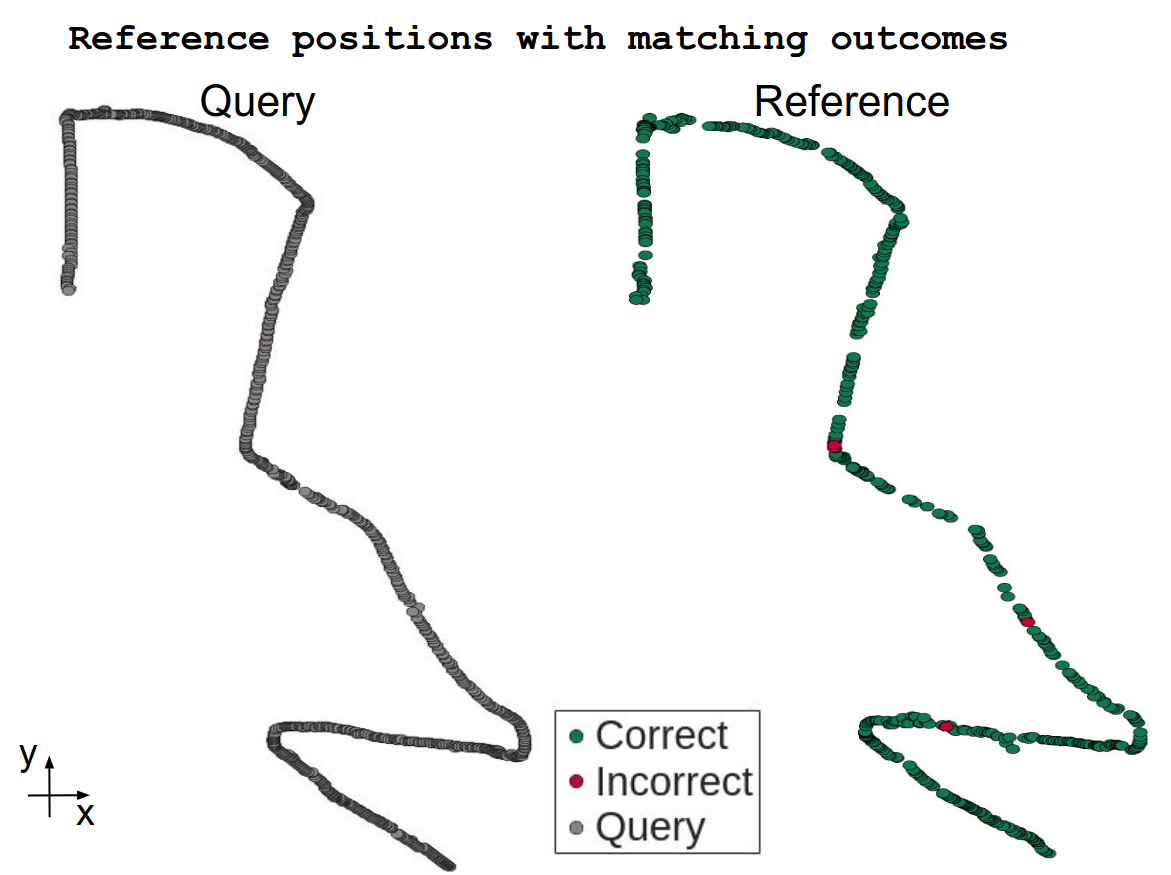
\includegraphics[width=0.9\linewidth]{images/positions_test.png}
    \caption{Matching outcomes for retrieved reference samples.}
    \label{fig:positions_test}
\end{figure}


%, however, it still ranks among the top three in precision when combined with the Cosplace descriptor. In sum, considering all data sets in Table~\ref{tab:short_results}, Synthia was the only one where normalization seems to have a negative impact on performance.

% Notably, ST-LARFSOM combined with MixVPR achieves the best overall performance across all scenarios, except for the precision on Synthia, where it still sits for among the top three in terms of mF1. In this case, we observed that the performance varies depending on the shift applied to the query position data, though, a tolerance reduction caused STS-VPR outperformed the others. However, for comparison sake, we assigned the same configuration as in \cite{tolerance_synthia}. In spite this only setback, the overall results highlight the robustness of our approach under different contexts, including high appearance variation, as observed in EuRoC and in the day–night sequences of RobotCar; and in significant viewpoint changes, as in the Synthia and KITTI datasets with opposite camera perspectives.

% Falar sobre as médias
STS-VPR is a nonlinear system; hence, its dynamic depends on its initial state and the order of the presentations of the samples. Though, the average performance and the standard deviation values (see Table~\ref{tab:mean_precision}) suggest precision and robustness, \textit{i.e.}, the mean values of the dispersions are very regularly close to the corresponding maximum precision and mF1.

It is worth commenting on the use of Self-organizing Maps for VPR. Table~\ref{tab:short_results} shows that a previous attempt, the SOM-based categorizer SCMuSOM, struggled to reach the performance level of the models presented in this work. The fixed structure of the map, the uncontrolled degree of similarity between patterns of the same category, and the nonexistence of a normalization step seem to be the main reasons for the performance gaps. The first two points limit the map plasticity due to both the unawareness of the structure of the data set space and of a suitable size of the basins of attraction. The third feature weighs the balance of the ranges of components of the feature vectors. Therefore, the inserted mechanisms provoked performance gains, particularly in data sets with larger room for improvement. 
% For instance, on RobotCar with CosPlace, STS-VPR improves performance by up to 16 percentage points over a prior baseline of 36.54\%. 
% On average, STS-VPR ameliorates performance in all shorter sequences: $4.57\%$ in precision and $10.25\%$ in mF1.  
% ablation
For example, the ablation study shown in Table~\ref{tab:ablation} highlights the impact of inserting memory and normalization on the precision for LARFSOM using MixVPR as the feature extractor for two different data sets. Moreover, Fig. \ref{fig:ablation} illustrates the importance of temporal context in the recognition process by showing how considering previous images helps to remove ambiguity that may lead to a wrong match.

\begin{table}[t]
\centering
\caption{Ablation study of LARFSOM using MixVPR for feature extraction, comparing maximum precision of LARFSOM against LARFSOM with short tem memory (STM) and LARFSOM with STM and normalization.}
\label{tab:ablation}
\begin{tabular}{lccc}
\hline
\textbf{} & \textbf{Robotcar} & \textbf{Euroc} \\
\hline
LARFSOM          & 97.12 & 84.27 \\

LARFSOM with STM   & 99.40 & 87.75 \\
LARFSOM with STM and normalization & 99.60 & 89.57 \\

\hline
\end{tabular}

\end{table}




\begin{figure}[ht]   

    \caption{\DIFdelbeginFL \DIFdelFL{Illustration of the role of temporal context in ST-LARFSOM. For the same query image, only }\DIFdelendFL ST-LARFSOM correctly disambiguates the match \DIFaddbeginFL \DIFaddFL{using temporal context}\DIFaddendFL , \DIFdelbeginFL \DIFdelFL{whereas }\DIFdelendFL \DIFaddbeginFL \DIFaddFL{unlike }\DIFaddendFL LARFSOM\DIFdelbeginFL \DIFdelFL{fails due to the absence of contextual information}\DIFdelendFL .}
    \label{fig:ablation}
    \centering
    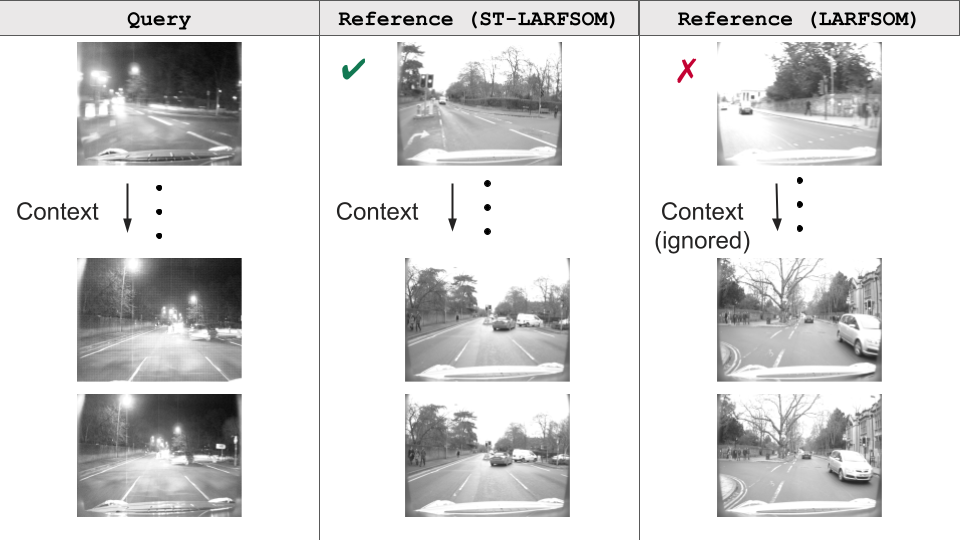
\includegraphics[width=1\columnwidth]{images/context.png}
\end{figure}

% Falar sobre o tempo de execução para estas mesmas sequências
Although ST-LARFSOM is not always the top performer in terms of accuracy, it consistently achieves significantly lower matching times in all data sets. Table~\ref{tab:times} shows the total processing time, including the matching and feature extraction stages (or preprocessing for SeqSLAM). While the total computation time for shorter sequences may not differ largely, there are bold cases, such as the Kitti data set, where STS-VPR can be approximately 3 times faster in the overall processing when compared with the respective descriptor. The difference increases when compared against older models.

%%%%%%%%%%%%%%%%%%%%%%%%%%%%%%%
\subsubsection{Long sequences}

% Falar sobre a precisão e mF1 e precisão em 100% de recall para as menores sequências
To complete our evaluation of the proposed model, additional tests were carried out with sequences containing a larger number of images (more than 10,000 samples). We first consider the Robotcar data set, which is subdivided into three sequence pairs (1, 2, and 3), all using 09/12/2014 (day) as the reference and 10/12/2014 (night), 14/11/2014 (night) and 13/02/2015 (day) as the queries. The precision and mF1 scores are shown in Table~\ref{tab:long_results} \footnote{There are no results for MPF, as its RAM consumption made the matching process infeasible on the used machine.}. 
%
For pairs 1 and 2, the STS-VPR methods show an average increase in precision and mF1 compared to other approaches. For pair 3, the results show a similar precision with a small decrease for the mF1 score. This is due to the initially very high performance of the other methods, which leaves little room for improvement. This part of the sequence consists of images sufficiently distinct from each other that contextualization is not necessary. These results are consistent when considering the mean and standard deviation presented in Table \ref{tab:mean_precision_long}. The main difference lies in the computation time (see Table \ref{tab:times_long}). Indeed, with long sequences containing numerous images, the proposed approach significantly reduces computation time, between 4 and 6 times faster.

%  Except for Pitts30k and Nordland, STS-VPR matches
% or outperforms all competing methods. Overall, it shows an average $3.61\%$ gain in precision and $1.33\%$ in mF1.

Regarding the Nordland data set, the performance remains competitive.
During training, ST-LARFSOM required a larger number of epochs to reduce the unsupervised error below the threshold $\delta_{th}$, indicating a more competitive scenario; nevertheless, the temporal context remains effective as a disambiguating factor. Notably, Nordland is the only data set in which SeqSLAM outperforms all other models, likely due to its favorable acquisition conditions: images are captured from a train moving at nearly constant speed with minimal viewpoint variation.

% falar do pitts30k
Finally, we consider the results obtained with the Pitts30k data set. As can be seen in Table \ref{tab:precision_mf1_long}, the precision and mF1 scores are significantly lower for the STS-VPR methods. This can be explained by the nature of the data set. It is made of short sequences of images (approximately 24) of the same place, concatenated one after the other. During the construction of the spatio-temporal feature vector, the short-term memory process might use images from two different places. This is an extreme example of the limitation of such memory. \DIFdelbegin \DIFdel{We could also mention the case of a }\DIFdelend \DIFaddbegin \DIFadd{In addition, another limitation arises when the }\DIFaddend short-term memory \DIFdelbegin \DIFdel{made of a unique }\DIFdelend \DIFaddbegin \DIFadd{contains a single }\DIFaddend image captured while the \DIFdelbegin \DIFdel{car was stopped }\DIFdelend \DIFaddbegin \DIFadd{vehicle is stationary (e.g., }\DIFaddend at a traffic light\DIFdelbegin \DIFdel{compared with }\DIFdelend \DIFaddbegin \DIFadd{), as opposed to }\DIFaddend a sequence of \DIFaddbegin \DIFadd{visually }\DIFaddend distinct images captured while the \DIFdelbegin \DIFdel{car was driving at the exact same place. It }\DIFdelend \DIFaddbegin \DIFadd{vehicle is moving through the same location. Therefore, it }\DIFaddend will then be necessary in future works to explore how the images selected by the short-term memory process must be selected to avoid the aforementioned issues.

% In general, when a reference sequence is matched against itself, the first 90 images fall within the tolerance before the first incorrect match occurs. In contrast, for Pitts30k, only the first 13 images satisfy the tolerance on average. However, considering solely the geometric ordering of Pitts30k, up to 196 images should lie within tolerance regardless of matching. This discrepancy explains the performance degradation observed in these experiments: for Pitts30k, the descriptors retrieve substantially fewer valid candidates than the tolerance would allow. Consequently, clustering without performance loss becomes infeasible, as the scarcity of valid matches leads to incorrect groupings. Table~\ref{tab:mean_precision_long} further shows that these results are robust to stochasticity, with Pitts30k being the only exception.

% Falar sobre o tempo de execução para estas mesmas sequências
Table~\ref{tab:times_long} confirms that STS-VPR can scale, showing the
suitability of using ST-LARFSOM in the matching process. A prominent example
was reached by the combination ST-LARFSOM with Cosplace feature extractor
that responded within a matching time up to 42$\times$ faster than the second
pair in the Oxford Robotcar data set, and remained up to 4$\times$ faster when
feature extraction time was also considered. The consistent and significant
improvements over different models and data sets suggest that the time
reduction becomes more pronounced when the size of the reference set
increases, further reinforcing the scalability of our approach.


%- Pitts 30k e Nordland são os data sets com menor dispersão;

%- resultados piores em Pitts 30k não tem a ver com a normalização;

%%%%%%%%%%%%%%%%%%%%%
\section{Conclusion}

\begin{figure}[ht]   

    \caption{Successful matching occurrences on different data sets.}
    \label{fig:qualitative}
    \centering
    \includegraphics[width=1\columnwidth]{images/qualitative.png}
\end{figure}

A novel VPR model is proposed, which leverages adaptive clustering to
significantly reduce computation time, reducing up to 42$\times$ the matching
speed when compared with other models. STS-VPR employs temporal and
normalized feature descriptors combined with a \ac{SOM-TVS}, which
dynamically adapts its structure to new inputs by clustering the most similar
samples. This matching procedure compares a query vector with a subset of reference vectors \DIFdelbegin \DIFdel{, those in }\DIFdelend \DIFaddbegin \DIFadd{within }\DIFaddend the winner group.

The tests suggest improvements in computational efficiency and in precision in comparison with prior models. The LARFSOM was already competitive without considering the STM formulation, but the precision gain derives mainly from this spatio-temporal representation; normalization-based saturation only refines it and must be applied after STM aggregation. Fig.~\ref{fig:qualitative} \DIFdelbegin \DIFdel{shows the challenging data sets }\DIFdelend \DIFaddbegin \DIFadd{illustrates several challenging cases }\DIFaddend on which our model was evaluated, including conditions such as seasonal changes, day–night variations, and large viewpoint shifts\DIFdelbegin \DIFdel{. Fig.~\ref{fig:qualitative} illustrates the challenging datasets used (seasonal shifts, day–night changes, large viewpoint variations)}\DIFdelend .

%%% Maybe this was not relevant (removing because of space)
%Applying saturation beforehand prematurely clips descriptor variance, removing information needed to form temporal context and thereby degrading the STM’s ability to encode temporal relationships, sometimes producing worse representations than no normalization.

Future work may investigate the application of this network in real-time scenarios to compare its performance against existing approaches. Additional research could also explore strategies to reduce training complexity, potentially enabling online learning in which past query images serve as references. Finally, further mechanisms may be introduced to minimize or eliminate the model’s dependence on sensitive hyperparameters.

\bibliographystyle{IEEEtran.bst}
\bibliography{IEEEexample}


\end{document}
